% Welcome! This is the unofficial University of Udine beamer template.

% See README.md for more informations about this template.

% This style has been developed following the "Manuale di Stile"
% (Style Manual) of the University of Udine. You can find the
% manual here: https://www.uniud.it/it/ateneo-uniud/ateneo-uniud/identita-visiva/manuali-immagine-stile/manuale-stile

% Note: for some reason, the RGB values specified in the manual
% do NOT render correctly in Beamer, so they have been redefined
% for this document using the high level chromo-optic deep neural 
% quantistic technology offered by Microsoft Paint's color picker.

% We defined four theme colors: UniBrown, UniBlue, UniGold
% and UniOrange. For example, to write some uniud-brownish
% text, just use: \textcolor{UniBrown}{Hello!}

% Note that [usenames,dvipsnames] is MANDATORY due to compatibility
% issues between tikz and xcolor packages.

\documentclass[usenames,dvipsnames]{beamer}
\usepackage[utf8]{inputenc}
\usepackage{verbatim}
\usepackage{multicol}
\usepackage{cases}
\usepackage{cancel}
\usetheme{uniud}
%set depth of Outline
\setcounter{tocdepth}{2}
%%% Bibliography
\usepackage[style=authoryear,backend=biber]{biblatex}
\addbibresource{bibliography.bib}

% Author names in publication list are consistent 
% i.e. name1 surname1, name2 surname2
% See https://tex.stackexchange.com/questions/106914/biblatex-does-not-reverse-the-first-and-last-names-of-the-second-author
\DeclareNameAlias{author}{first-last}

%%% Suppress biblatex annoying warning
\usepackage{silence}
\WarningFilter{biblatex}{Patching footnotes failed}

%%% Some useful commands
% pdf-friendly newline in links
\newcommand{\pdfnewline}{\texorpdfstring{\newline}{ }} 
% Fill the vertical space in a slide (to put text at the bottom)
\newcommand{\framefill}{\vskip0pt plus 1filll}


\title[IHEP SUSY Group Meeting]{Group Meeting}
\date[Oct 23, 2024]{Oct 23, 2024}
\author[Chengxin Liao]{
  Chengxin Liao
  \pdfnewline
  \texttt{lcx1937629829@icloud.com}
}
\institute{Department of Physics, Shandong University}

\begin{document}

\begin{frame}
\titlepage
\end{frame}

\begin{frame}{Outline}
\tableofcontents
\end{frame}

\section{C1N2ISR:introduction}
\subsection{selection}
\begin{frame}
\frametitle{C1N2ISR:introduction}
\framesubtitle{selection}
\begin{columns}
    \column{0.6\textwidth}
    \raggedright
    Selection

    lep-had channel:nTaus$\geq$1;nLeps$\geq$1
    
    had-had channel:nTaus$\geq$2;nLeps=0
    
    MET$\geq$ 200; pass MET trigger
    
    $1\leq nBaseJet\leq 8$
     
    b-veto
    
    OS
    \vskip 0.2cm
    
    For sig/bkg plot, both bkg and signal distribution are normalized to 1.
    \column{0.5\textwidth}
    
    \raggedleft
    \begin{figure}
    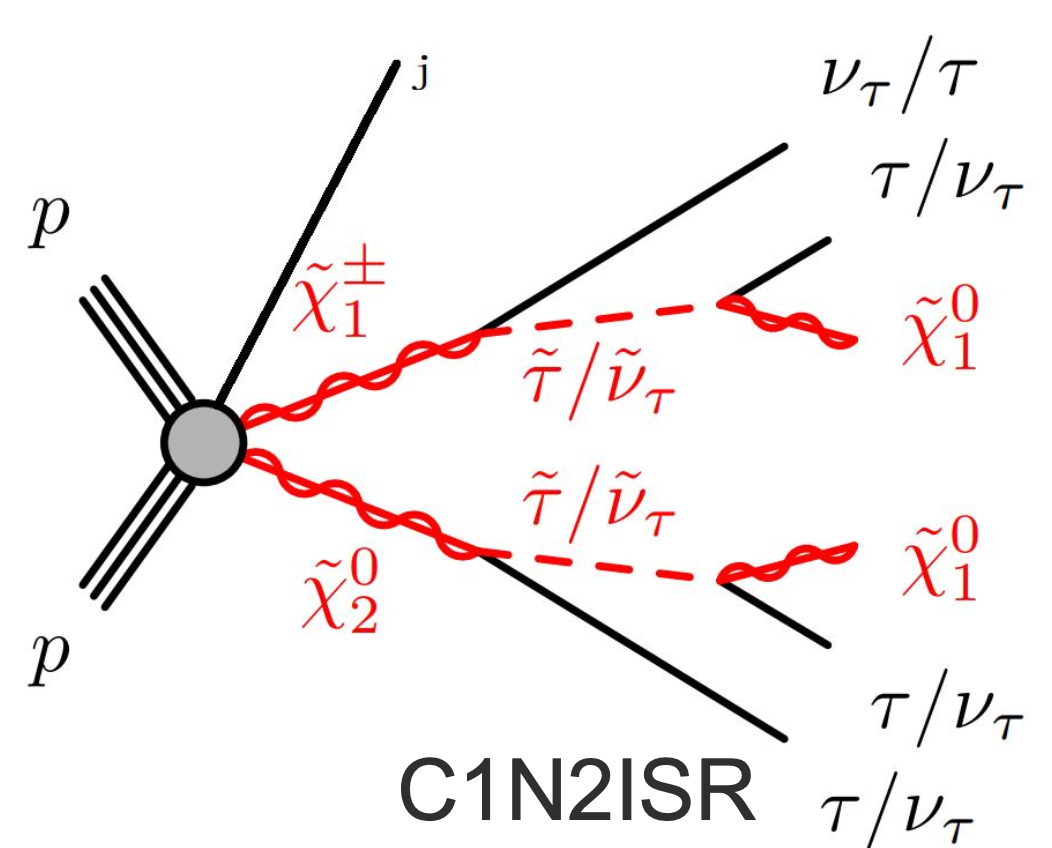
\includegraphics[width = 0.5\textwidth]{graphics/Feynman diagram.png}
    \end{figure}
 \end{columns}

\end{frame}

\section{C1N2ISR:MC modeling}
\subsection{cutflow check}
\begin{frame}
	\frametitle{C1N2ISR:MC modeling}
	\framesubtitle{HH cutflow check}
	jiarong's cutflow
	\begin{table}[!ht]
    \centering
    \resizebox{\textwidth}{!}{
    \begin{tabular}{|l|l|l|l|l|l|}
    \hline
        Cut name & baseline & signal tau cut & signal lep cut & pass MET trigger & MET>200 \\ \hline
        Wjets & 36910790.2 +- 22959.74 & 227485.23 +- 1770.31 & 73392.93 +- 955.13 & 37276.94 +- 471.71 & 4171.35 +- 75.96 \\ \hline
        TopPair & 7534021.4 +- 1055.09 & 46602.11 +- 85.24 & 29154.71 +- 68.3 & 25781.67 +- 63.35 & 3493.17 +- 23.03 \\ \hline
        SingleTop & 988110.24 +- 342.8 & 5067.94 +- 25.6 & 3222.52 +- 20.5 & 2828.31 +- 19.29 & 462.65 +- 8.04 \\ \hline
        OtherTop & 43746.18 +- 352.34 & 630.78 +- 22.85 & 273.86 +- 1.89 & 239.66 +- 1.8 & 55.96 +- 0.9 \\ \hline
        Zttjets & 5779690.55 +- 9204.86 & 70018.94 +- 785.84 & 42543.37 +- 548.16 & 23154.34 +- 161.89 & 2358.25 +- 29.33 \\ \hline
        Zlljets & 221114969.3 +- 28905.76 & 36458.71 +- 324.32 & 4319.3 +- 120.41 & 395.08 +- 4.87 & 61.84 +- 1.07 \\ \hline
        VV & 1310870.13 +- 2148.26 & 7533.16 +- 24.19 & 3139.54 +- 13.46 & 2621.95 +- 11.2 & 579.74 +- 4.12 \\ \hline
        Higgs & 29153.2 +- 18.17 & 867.06 +- 2.66 & 529.49 +- 1.91 & 402.02 +- 1.49 & 62.7 +- 0.6 \\ \hline
        dijet & 2739992885.1 +- 382761122.33 & 27609529.58 +- 26367725.95 & 27605283.03 +- 26367725.82 & 27535064.53 +- 26367714.5 & 186.17 +- 47.22 \\ \hline
        bkg & 3013704236.3 +- 382761124.23 & 28004193.52 +- 26367726.02 & 27761858.74 +- 26367725.84 & 27627764.5 +- 26367714.5 & 11431.82 +- 97.34 \\ \hline
        bkg wo dijet & 273711351.21 +- 38123.38 & 394663.94 +- 1966.15 & 156575.71 +- 1110.19 & 92699.97 +- 503.25 & 11245.65 +- 85.12 \\ \hline
        data & 293007279.0 +- 17117.46 & 587437.0 +- 766.44 & 408035.0 +- 638.78 & 182497.0 +- 427.2 & 11234.0 +- 105.99 \\ \hline
    \end{tabular}
    }
\end{table}

	chengxin's cutflow
	\begin{table}[!ht]
    \centering
    \resizebox{\textwidth}{!}{
    \begin{tabular}{|l|l|l|l|l|l|}
    \hline
        Cut name & baseline & signal tau cut & signal lep cut & pass MET trigger & MET>150 \\ \hline
        Wjets & 36922766.96 +- 22960.52 & 227485.23 +- 1770.31 & 73392.93 +- 955.13 & 37276.94 +- 471.71 & 11976.76 +- 189.99 \\ \hline
        TopPair & 7543957.29 +- 1055.81 & 46602.11 +- 85.24 & 29154.71 +- 68.3 & 25781.67 +- 63.35 & 9935.89 +- 38.89 \\ \hline
        SingleTop & 989268.38 +- 343.03 & 5067.94 +- 25.6 & 3222.52 +- 20.5 & 2828.31 +- 19.29 & 1158.14 +- 12.52 \\ \hline
        OtherTop & 43867.26 +- 352.34 & 630.78 +- 22.85 & 273.86 +- 1.89 & 239.66 +- 1.8 & 121.07 +- 1.3 \\ \hline
        Zttjets & 5786808.72 +- 9205.01 & 70018.94 +- 785.84 & 42543.37 +- 548.16 & 23154.34 +- 161.89 & 7118.17 +- 52.53 \\ \hline
        Zlljets & 221115127.81 +- 28905.76 & 36458.71 +- 324.32 & 4319.3 +- 120.41 & 395.08 +- 4.87 & 158.51 +- 2.03 \\ \hline
        VV & 1312106.56 +- 2148.27 & 7533.16 +- 24.19 & 3139.54 +- 13.46 & 2621.95 +- 11.2 & 1236.43 +- 6.55 \\ \hline
        Higgs & 29318.3 +- 18.19 & 867.06 +- 2.66 & 529.49 +- 1.91 & 402.02 +- 1.49 & 165.1 +- 0.96 \\ \hline
        dijet & 2739993771.09 +- 382761122.33 & 27609529.58 +- 26367725.95 & 27605283.03 +- 26367725.82 & 27535064.53 +- 26367714.5 & 885.99 +- 206.95 \\ \hline
        bkg & 3013736992.37 +- 382761124.23 & 28004193.52 +- 26367726.02 & 27761858.74 +- 26367725.84 & 27627764.5 +- 26367714.5 & 32756.06 +- 288.8 \\ \hline
        bkg wo dijet & 273743221.27 +- 38123.91 & 394663.94 +- 1966.15 & 156575.71 +- 1110.19 & 92699.97 +- 503.25 & 31870.07 +- 201.43 \\ \hline
        data & 292645456.0 +- 17106.88 & 586282.0 +- 765.69 & 407240.0 +- 638.15 & 182101.0 +- 426.73 & 31921.0 +- 178.66 \\ \hline
    \end{tabular}
    }
\end{table}
\end{frame}

\begin{frame}
\frametitle{C1N2ISR:MC modeling}
\framesubtitle{HH cutflow check}
jiarong's cutflow(hhmetrun2)
\begin{figure}
	\centering
	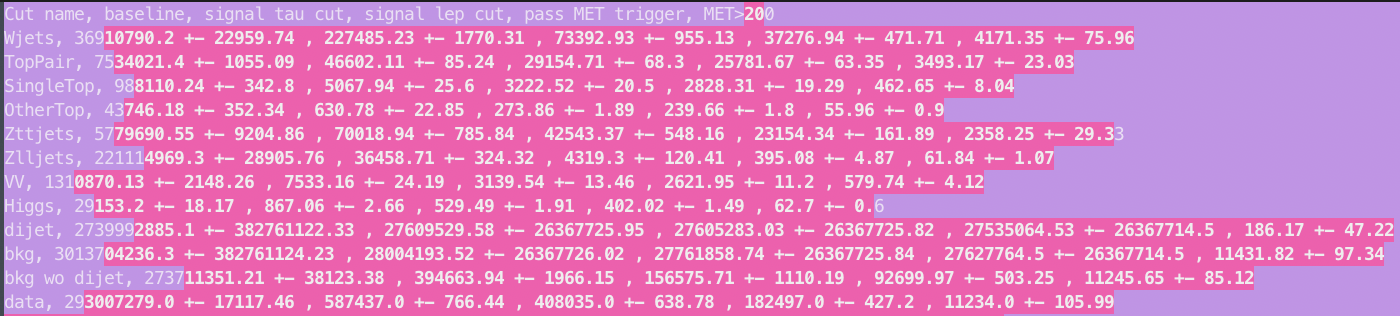
\includegraphics[width = 0.9\textwidth]{graphics/jiaronghhcutflow}
	\label{jiarong's hh cutflow}
\end{figure}
chengxin;s cutflow
\begin{figure}
	\centering
	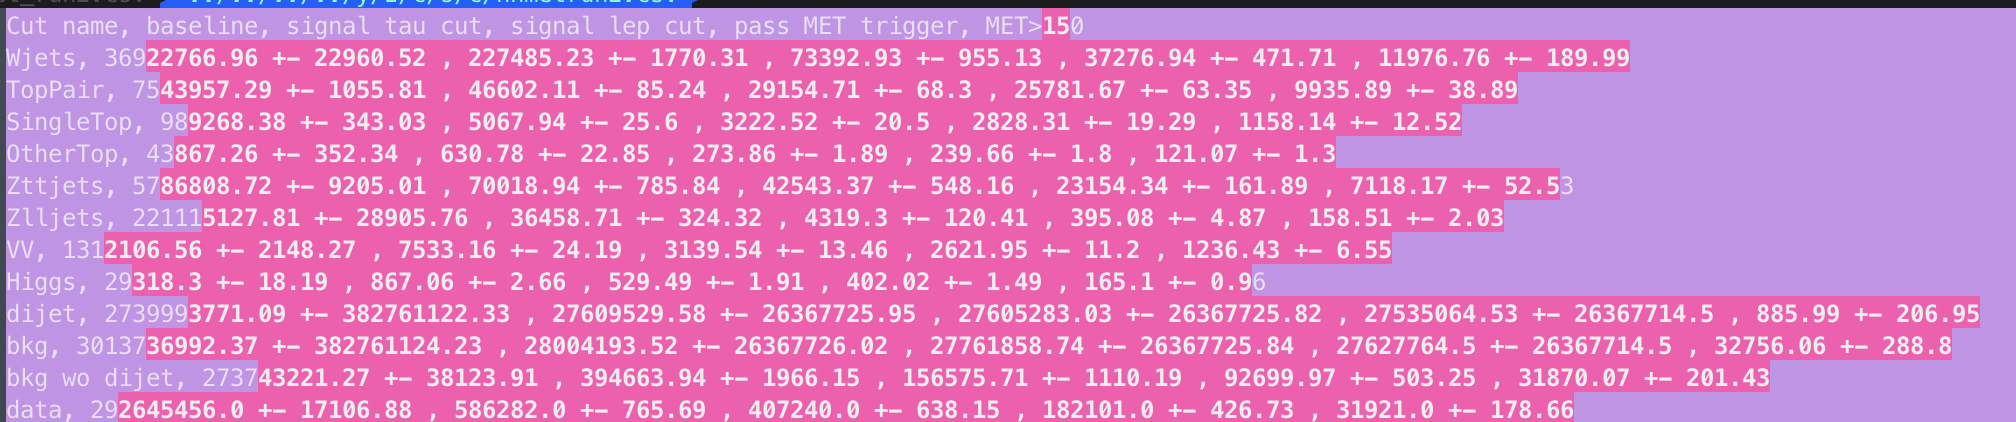
\includegraphics[width = 0.9\textwidth]{graphics/chengxinhhcutflow}
	\label{chengxin's hh cutflow}
\end{figure}
\end{frame}

\begin{frame}
	\frametitle{C1N2ISR:MC modeling}
	\framesubtitle{LH cutflow check}
	jiarong's cutflow
	\begin{table}[!ht]
    \centering
    \resizebox{\textwidth}{!}{
    \begin{tabular}{|l|l|l|l|l|l|}
    \hline
        Cut name & baseline & signal tau cut & signal lep cut & pass MET trigger & MET>200 \\ \hline
        Wjets & 36910790.2 +- 22959.74 & 20163118.47 +- 17726.83 & 19181417.03 +- 17321.41 & 400339.22 +- 855.46 & 19908.53 +- 106.14 \\ \hline
        TopPair & 7534021.4 +- 1055.09 & 1512883.18 +- 476.74 & 1274946.24 +- 434.67 & 325111.94 +- 220.23 & 28971.03 +- 65.77 \\ \hline
        SingleTop & 988110.24 +- 342.8 & 201833.19 +- 155.94 & 175293.87 +- 144.99 & 34093.54 +- 66.93 & 3313.02 +- 21.4 \\ \hline
        OtherTop & 43746.18 +- 352.34 & 8482.23 +- 152.45 & 5767.05 +- 135.27 & 2399.01 +- 91.23 & 432.14 +- 20.72 \\ \hline
        Zttjets & 5779690.55 +- 9204.86 & 3220731.18 +- 6973.12 & 2637387.66 +- 6459.62 & 70581.09 +- 341.53 & 4334.14 +- 38.75 \\ \hline
        Zlljets & 221361064.12 +- 28909.58 & 4059890.39 +- 4073.07 & 2078249.12 +- 3279.28 & 17064.81 +- 72.84 & 265.74 +- 3.81 \\ \hline
        VV & 1310870.13 +- 2148.26 & 221902.39 +- 765.78 & 183041.15 +- 176.22 & 24420.22 +- 37.63 & 3753.33 +- 9.85 \\ \hline
        Higgs & 29153.2 +- 18.17 & 23663.9 +- 17.51 & 18105.11 +- 15.51 & 1913.19 +- 4.55 & 180.64 +- 1.41 \\ \hline
        dijet & 2739992885.1 +- 382761122.33 & 207700675.42 +- 54043947.9 & 93288309.52 +- 32863616.64 & 17425.83 +- 4207.3 & 118.82 +- 35.7 \\ \hline
        bkg & 3013950331.12 +- 382761124.23 & 237113180.35 +- 54043951.42 & 118842516.75 +- 32863622.01 & 893348.86 +- 4314.85 & 61277.38 +- 139.17 \\ \hline
        bkg wo dijet & 273957446.02 +- 38126.27 & 29412504.93 +- 19501.7 & 25554207.23 +- 18782.2 & 875923.03 +- 957.34 & 61158.56 +- 134.51 \\ \hline
        data & 292613535.0 +- 17105.95 & 31554940.0 +- 5617.38 & 24770923.0 +- 4977.04 & 739914.0 +- 860.18 & 54826.0 +- 234.15 \\ \hline
    \end{tabular}
    }
\end{table}

chengxin's cutflow
\begin{table}[!ht]
    \centering
    \resizebox{\textwidth}{!}{
    \begin{tabular}{|l|l|l|l|l|l|}
    \hline
        Cut name & baseline & signal tau cut & signal lep cut & pass MET trigger & MET>150 \\ \hline
        Wjets & 36973006.96 +- 22960.76 & 20163118.47 +- 17726.83 & 19197702.26 +- 17326.57 & 400852.5 +- 856.02 & 62216.76 +- 217.23 \\ \hline
        TopPair & 7620854.23 +- 1061.2 & 1512883.18 +- 476.74 & 1326081.89 +- 443.18 & 337671.69 +- 224.38 & 86832.83 +- 113.71 \\ \hline
        SingleTop & 996942.3 +- 344.54 & 201833.19 +- 155.94 & 179968.97 +- 147.21 & 35029.51 +- 67.91 & 8832.05 +- 34.5 \\ \hline
        OtherTop & 44817.59 +- 354.91 & 8482.23 +- 152.45 & 7283.24 +- 145.4 & 2953.46 +- 93.85 & 1071.41 +- 42.68 \\ \hline
        Zttjets & 5792900.21 +- 9205.45 & 3220731.18 +- 6973.12 & 2654322.19 +- 6473.64 & 71148.75 +- 341.96 & 13209.66 +- 104.45 \\ \hline
        Zlljets & 221115919.53 +- 28905.76 & 4055309.63 +- 4072.66 & 3950413.09 +- 4028.51 & 42308.0 +- 100.53 & 950.23 +- 9.06 \\ \hline
        VV & 1320120.19 +- 2273.18 & 221902.39 +- 765.78 & 205260.58 +- 764.09 & 28031.04 +- 743.99 & 9250.07 +- 743.18 \\ \hline
        Higgs & 29625.44 +- 18.31 & 23663.9 +- 17.51 & 18410.11 +- 15.57 & 1960.62 +- 4.59 & 472.24 +- 2.27 \\ \hline
        dijet & 2739993351.89 +- 382761122.33 & 207700675.42 +- 54043947.9 & 93294284.35 +- 32863616.87 & 17429.11 +- 4207.3 & 466.79 +- 118.86 \\ \hline
        bkg & 3013887538.35 +- 382761124.23 & 237108599.59 +- 54043951.42 & 120833726.69 +- 32863622.33 & 937384.67 +- 4379.33 & 183302.05 +- 800.35 \\ \hline
        bkg wo dijet & 273894186.46 +- 38131.59 & 29407924.17 +- 19501.62 & 27539442.34 +- 18951.78 & 919955.57 +- 1215.37 & 182835.25 +- 791.48 \\ \hline
        data & 292777737.0 +- 17110.75 & 31554940.0 +- 5617.38 & 26508997.0 +- 5148.69 & 776874.0 +- 881.4 & 164202.0 +- 405.22 \\ \hline
    \end{tabular}
    }
\end{table}
\end{frame}

\begin{frame}
\frametitle{C1N2ISR:MC modeling}
\framesubtitle{LH cutflow check}
jiarong's cutflow(lhmetrun2)
\begin{figure}
	\centering
	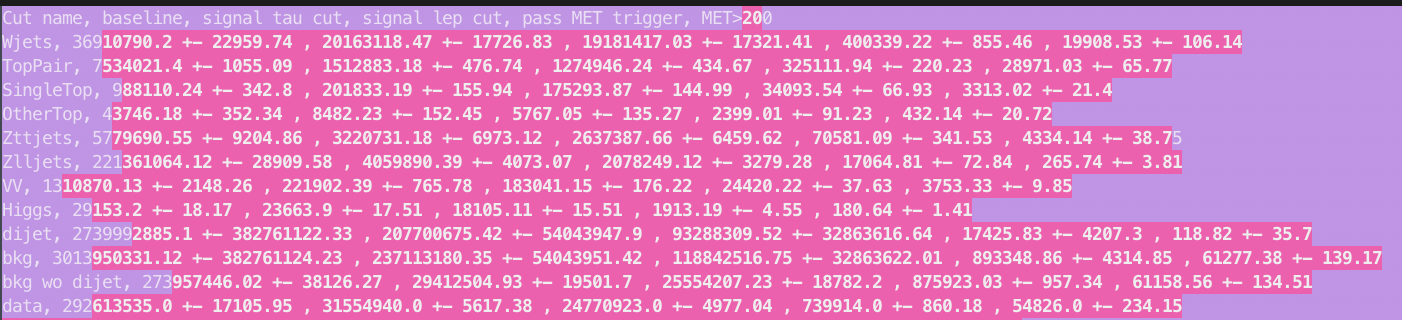
\includegraphics[width = 0.9\textwidth]{graphics/jiaronglhcutflow}
	\label{jiarong's lh cutflow}
\end{figure}
chengxin's cutflow
\begin{figure}
	\centering
	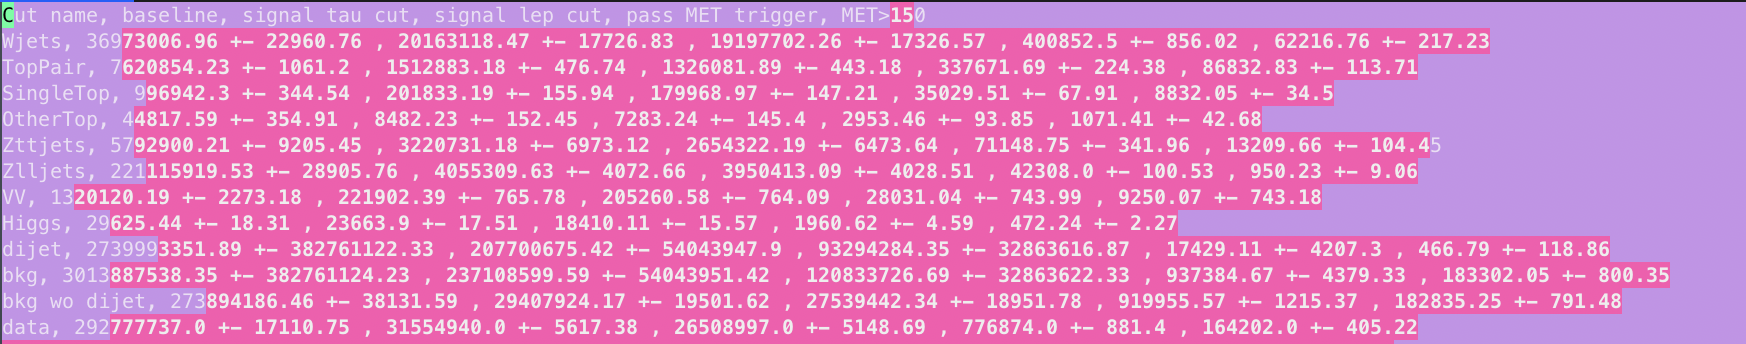
\includegraphics[width = 0.9\textwidth]{graphics/chengxinlhcutflow}
	\label{chengxin's lh cutflow}
\end{figure}
\end{frame}

\subsection{Normal Variable}
\begin{frame}
	\frametitle{C1N2ISR:MC modeling}
	\framesubtitle{Normal Variable}
	I put MC modeling plots in backup
\begin{equation*}
	variable:\left\{
	\begin{split}
		&\Delta\eta:\text{dEtat1j,dEtat2j,dEtatt}\\ 
		&\text{between tau1(tau2) and jet(tau2)}\\
		&\Delta\phi:dPhi(t1j,t1x,t2j,t2x,xj,tt)\\
		&\Delta R:dR(t1j,t1x,t2j,t2x,xj,tt),R = \sqrt{\Delta\eta^2 + \Delta\phi^2}\\
		&\eta:\eta(jet,lep,tau)\\
		&p_t:p_t(jet,lep,tau)\\
		&num:(\text{Jet,Ele,Muon,Tau,Lep,Tight Tau})\\
		&\text{transverse mass,stranverse mass:}\\
		&MET:Met, Metsig\\
		&\text{invariant mass}
	\end{split}
	\right.
\end{equation*}
\end{frame}

\subsection{mass distribution}
\begin{frame}
	\frametitle{C1N2:MC modeling}
	\framesubtitle{mass distribution}
	\begin{figure}
		\centering
		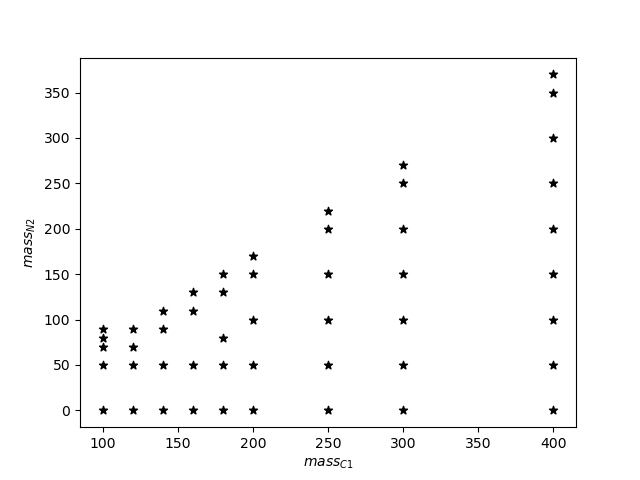
\includegraphics[width = 0.7\textwidth]{graphics/mass.png}
	\end{figure}
\end{frame}

\section{kinematic distribution}
\subsection{Variable choose}
\begin{frame}
	\frametitle{kinematic distribution}
	\framesubtitle{Variable choose}
		\begin{equation*}
		variable:
		\left\{
		\begin{split}
			& p_T:jet,lep,tau\\
      & MET\\
			& \text{num of obj}:base(jet,lep,e,\mu,\tau),\text{pass cut}(jet,lep,e,\mu,\tau,T\tau)\\
			& m_{inv}(tau1-tau2,t1-MET,t2-MET)\\
			& m_T:lep,jet,\tau,sum\\
			& MT2\\
			& ratio: \frac{jet}{tau1+tau2},\frac{jet}{tau1},\frac{jet}{tau2},\frac{MET}{tau1},\frac{MET}{tau2},\frac{MET}{tau1+tau2}\\
			& \Delta R: R_{t1-t2},R_{t1-E_{miss}},R_{t2-E_{miss}}, R_{t1-jet},R_{E_{miss}-jet}\\
			& \Delta \phi:\phi_{t1-t2},\phi_{t1-E_{miss}},\phi_{t2-E_{miss}}, \phi_{t1-jet},\phi_{E_{miss}-jet}
		\end{split}
		\right.
		\end{equation*}
\end{frame}

\subsection{LH kinematic distribution}
\begin{frame}
	\frametitle{kinematic distribution}
	\framesubtitle{LH:$p_T$}
% 第一行
    \begin{minipage}{0.32\textwidth}
        \centering
        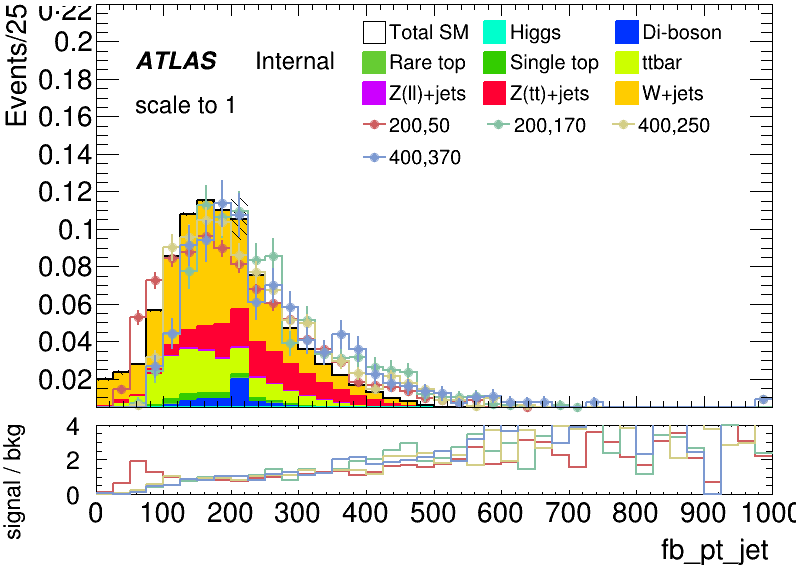
\includegraphics[width=\textwidth]{graphics/LH_met_sig/LH_fb_pt_jet_norm.png}
    \end{minipage}
    \hfill
    \begin{minipage}{0.32\textwidth}
        \centering
        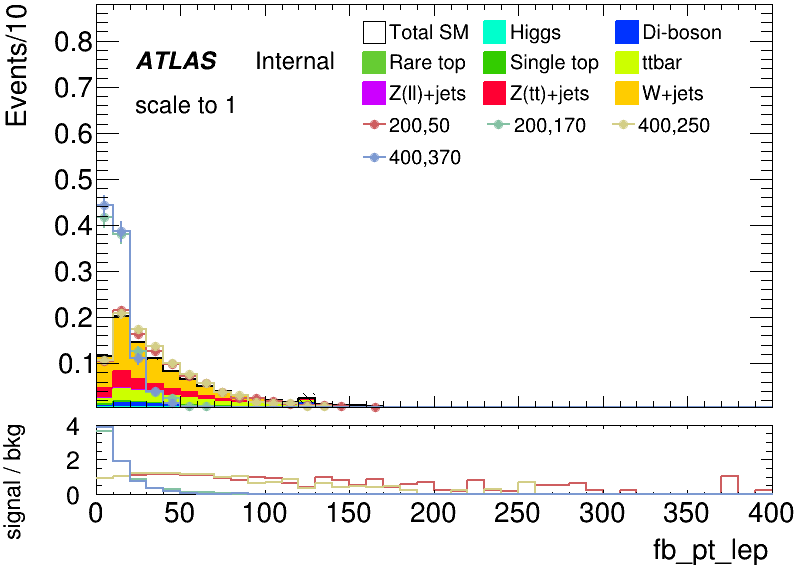
\includegraphics[width=\textwidth]{graphics/LH_met_sig/LH_fb_pt_lep_norm.png}
    \end{minipage}
    \hfill
    \begin{minipage}{0.32\textwidth}
        \centering
        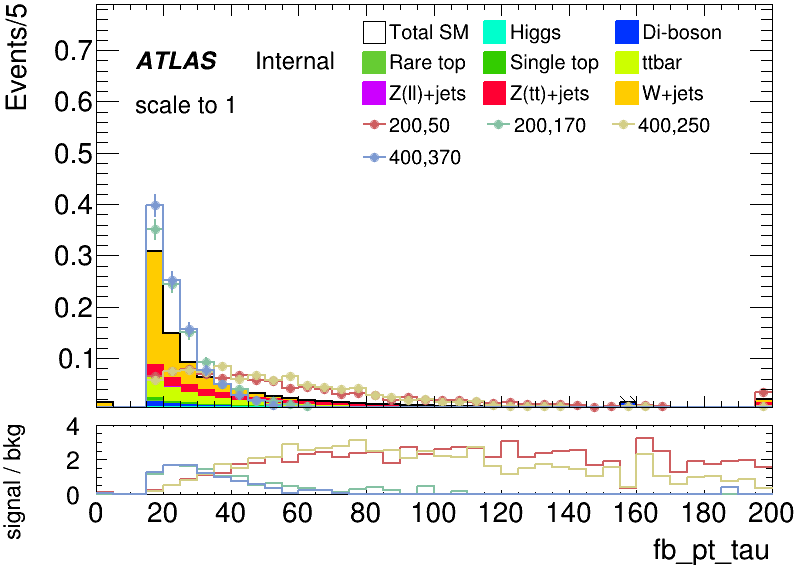
\includegraphics[width=\textwidth]{graphics/LH_met_sig/LH_fb_pt_tau_norm.png}
    \end{minipage}
    
    \vspace{0.5cm} % 图片之间的竖直间距
    
    notice: t1 is leading tau, t2 is leading lep, j is leading jet, x is MET.
\end{frame}

\begin{frame}
  \frametitle{kinematic distribution}
  \framesubtitle{LH:MET}
    \begin{minipage}{0.5\textwidth}
        \centering
        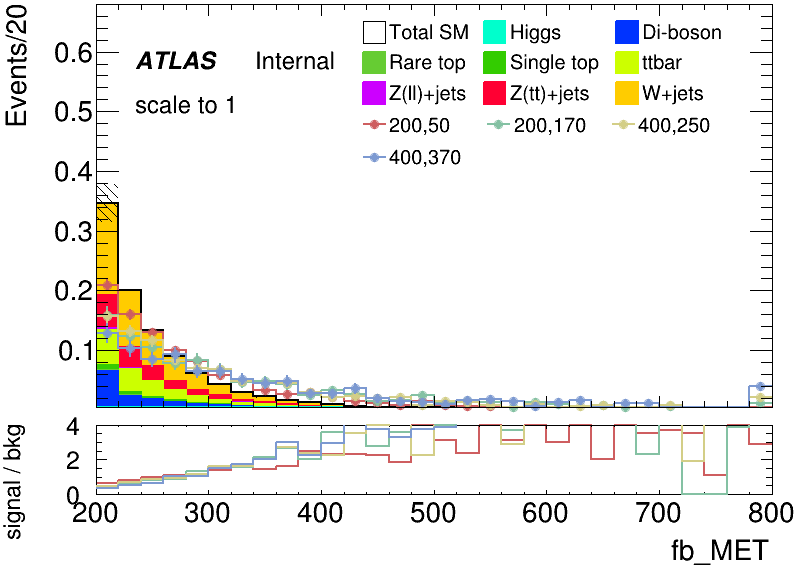
\includegraphics[width=\textwidth]{graphics/LH_met_sig/LH_fb_MET_norm.png}
    \end{minipage}
    \hfill
    \begin{minipage}{0.5\textwidth}
        \centering
        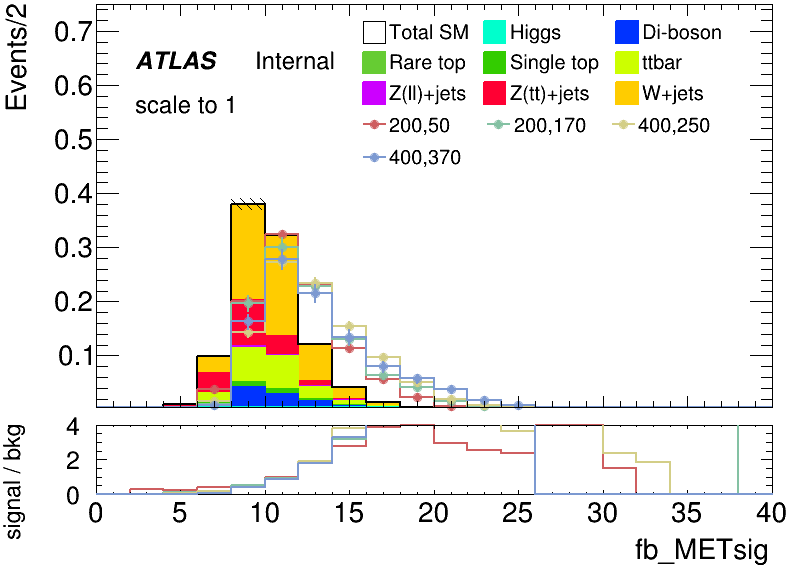
\includegraphics[width=\textwidth]{graphics/LH_met_sig/LH_fb_METsig_norm.png}
    \end{minipage}
\end{frame}

\begin{frame}
\frametitle{kinematic distribution}
\framesubtitle{LH:num of obj}
% 第一行
    \begin{minipage}{0.2\textwidth}
        \centering
        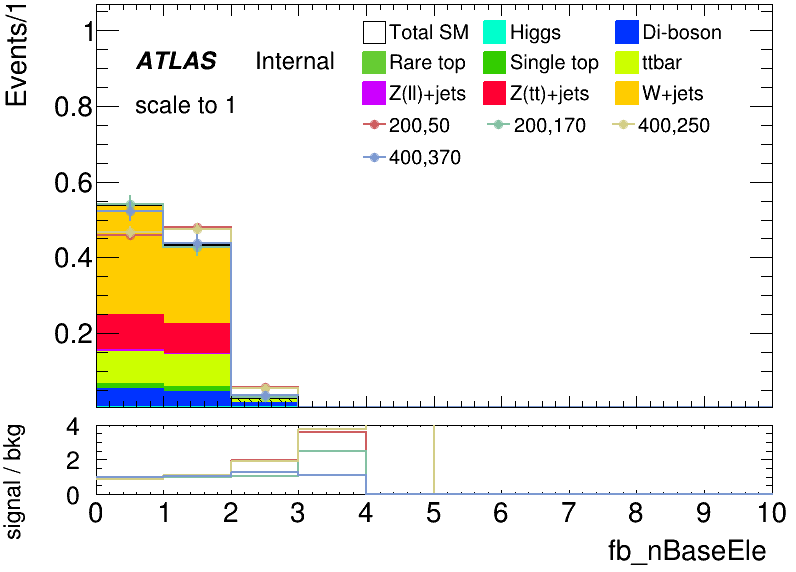
\includegraphics[width=\textwidth]{graphics/LH_met_sig/LH_fb_nBaseEle_norm.png}
    \end{minipage}
    \hfill
    \begin{minipage}{0.2\textwidth}
        \centering
        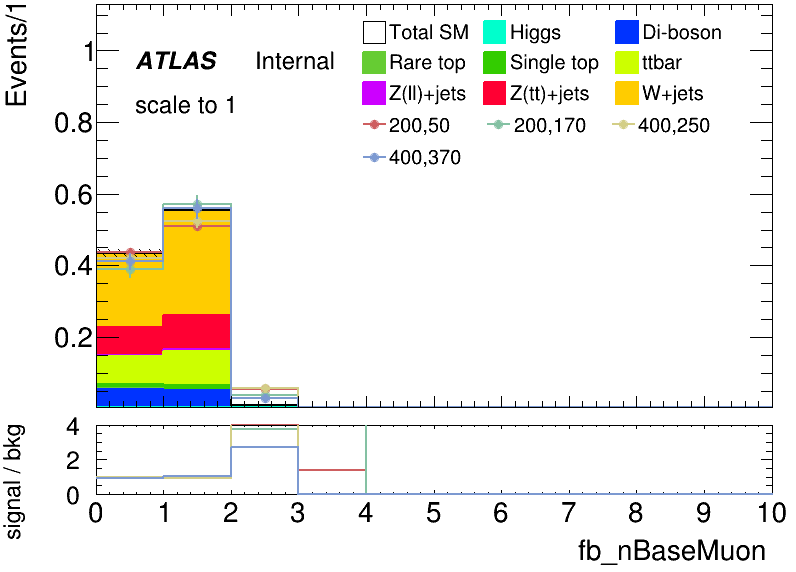
\includegraphics[width=\textwidth]{graphics/LH_met_sig/LH_fb_nBaseMuon_norm.png}
    \end{minipage}
    \hfill
    \begin{minipage}{0.2\textwidth}
        \centering
        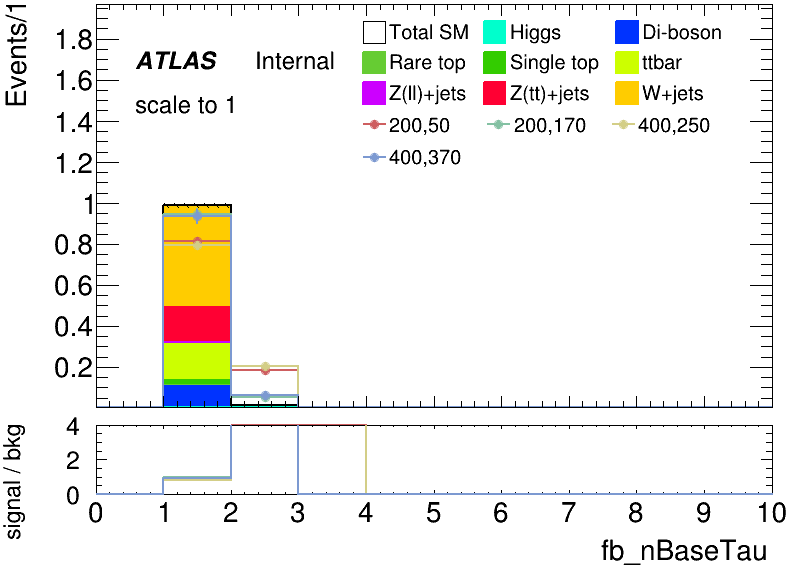
\includegraphics[width=\textwidth]{graphics/LH_met_sig/LH_fb_nBaseTau_norm.png}
    \end{minipage}
    \hfill
    \begin{minipage}{0.2\textwidth}
        \centering
        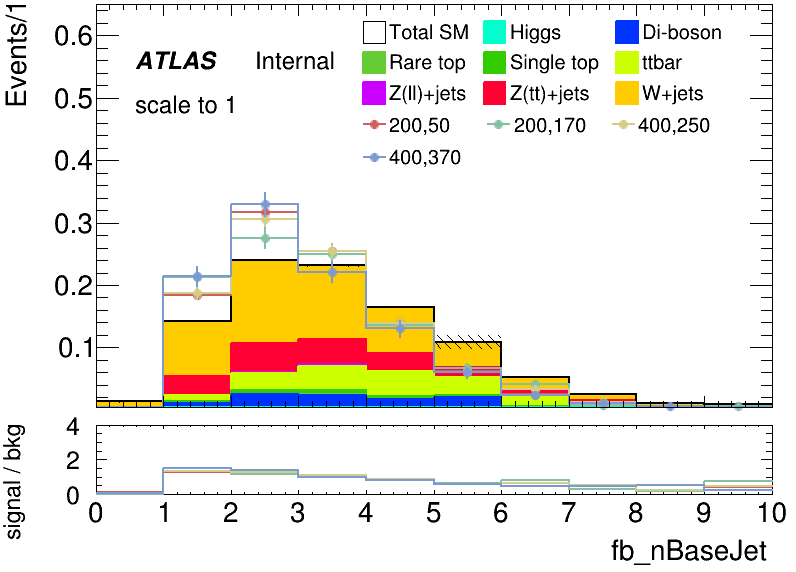
\includegraphics[width=\textwidth]{graphics/LH_met_sig/LH_fb_nBaseJet_norm.png}
    \end{minipage}
    \begin{minipage}{0.2\textwidth}
        \centering
        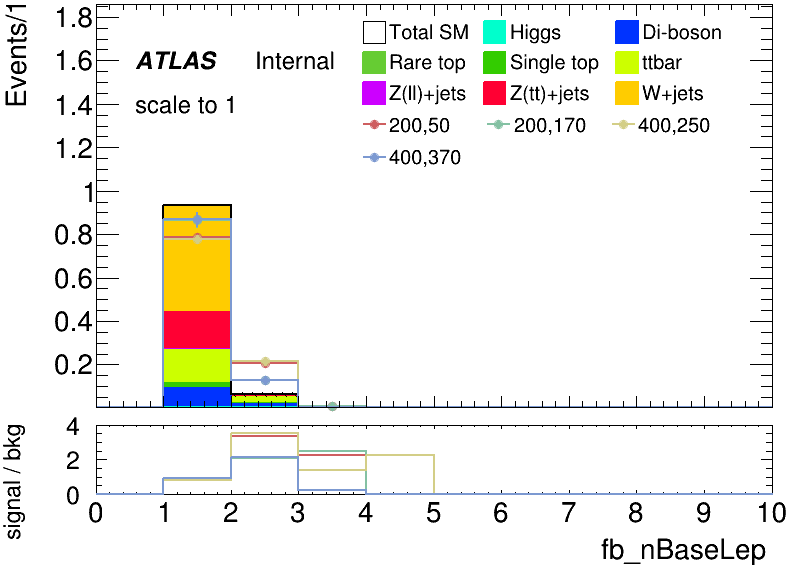
\includegraphics[width=\textwidth]{graphics/LH_met_sig/LH_fb_nBaseLep_norm.png}
    \end{minipage}
     
    \vspace{0.5cm} % 图片之间的竖直间距

    % 第二行
    \begin{minipage}{0.2\textwidth}
        \centering
        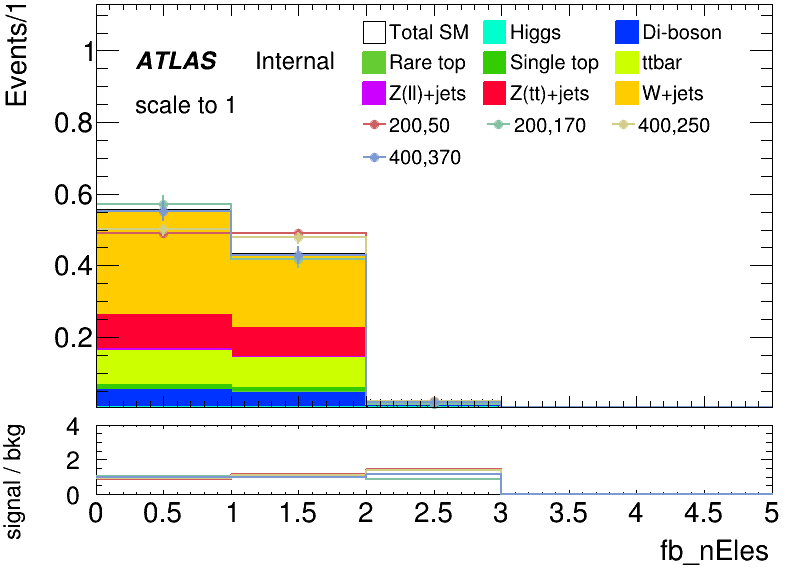
\includegraphics[width=\textwidth]{graphics/LH_met_sig/LH_fb_nEles_norm.png}
    \end{minipage}
    \hfill
    \begin{minipage}{0.2\textwidth}
        \centering
        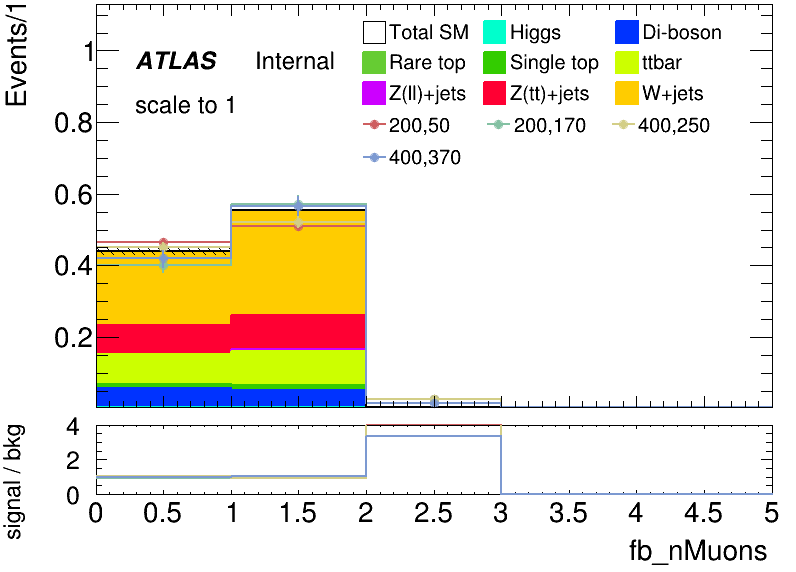
\includegraphics[width=\textwidth]{graphics/LH_met_sig/LH_fb_nMuons_norm.png}
    \end{minipage}
    \hfill
    \begin{minipage}{0.2\textwidth}
        \centering
        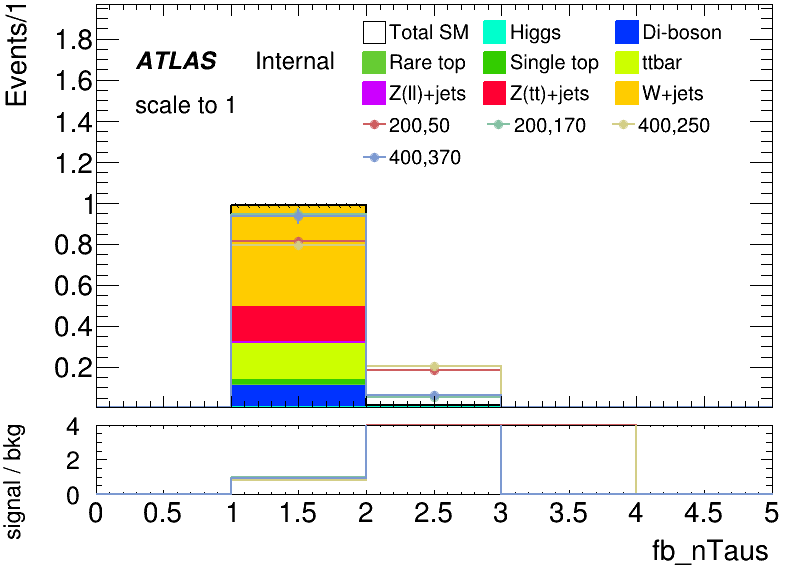
\includegraphics[width=\textwidth]{graphics/LH_met_sig/LH_fb_nTaus_norm.png}
    \end{minipage}
    \hfill
    \begin{minipage}{0.2\textwidth}
        \centering
        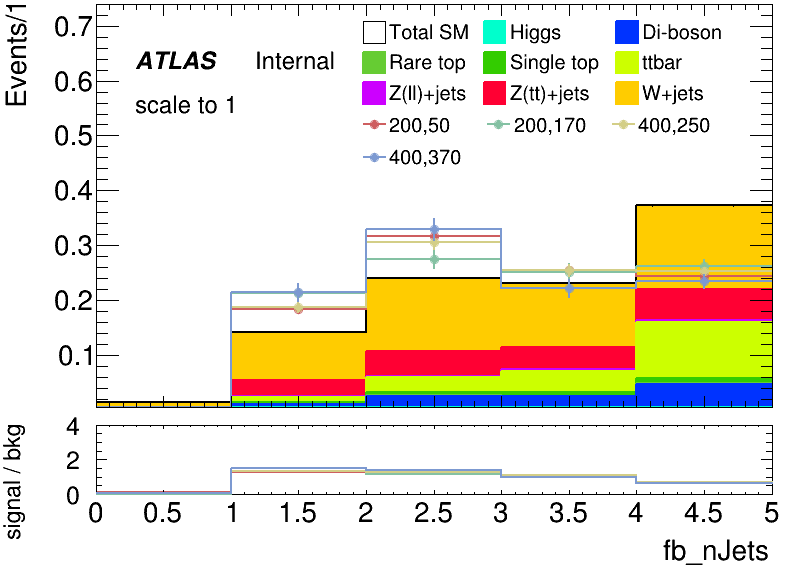
\includegraphics[width=\textwidth]{graphics/LH_met_sig/LH_fb_nJets_norm.png}
    \end{minipage}
    \begin{minipage}{0.2\textwidth}
        \centering
        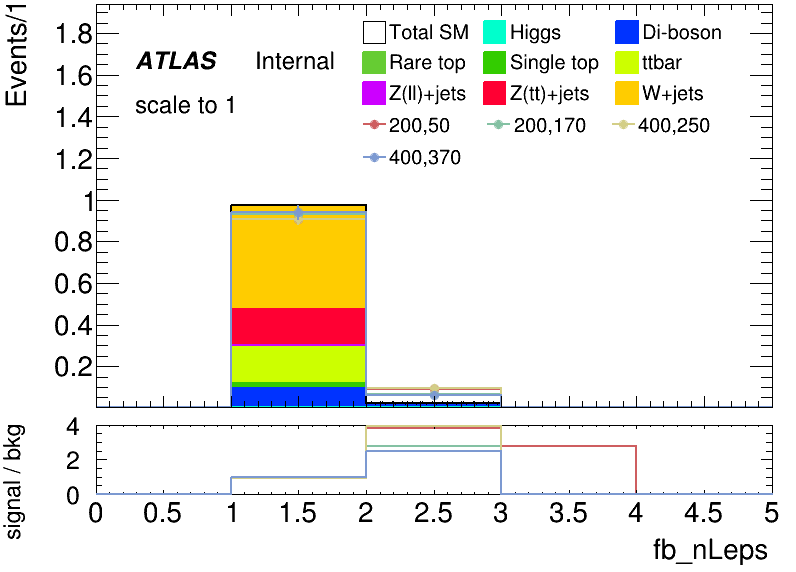
\includegraphics[width=\textwidth]{graphics/LH_met_sig/LH_fb_nLeps_norm.png}
    \end{minipage}
\end{frame}

\begin{frame}
	\frametitle{kinematic distribution}
	\framesubtitle{LH:num of obj}
	    \begin{minipage}{0.25\textwidth}
        \centering
        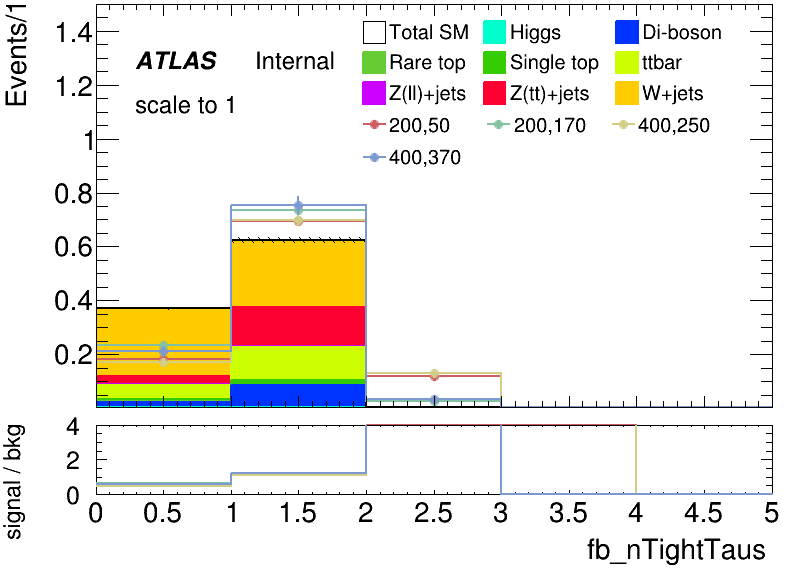
\includegraphics[width=\textwidth]{graphics/LH_met_sig/LH_fb_nTightTaus_norm.png}
    \end{minipage}
    \hfill
    \begin{minipage}{0.25\textwidth}
        \centering
        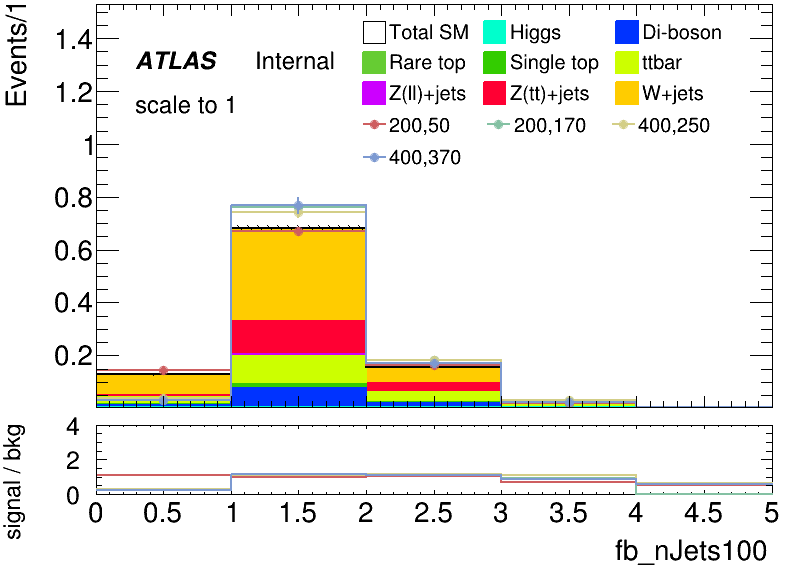
\includegraphics[width=\textwidth]{graphics/LH_met_sig/LH_fb_nJets100_norm.png}
    \end{minipage}
    \hfill
    \begin{minipage}{0.25\textwidth}
        \centering
        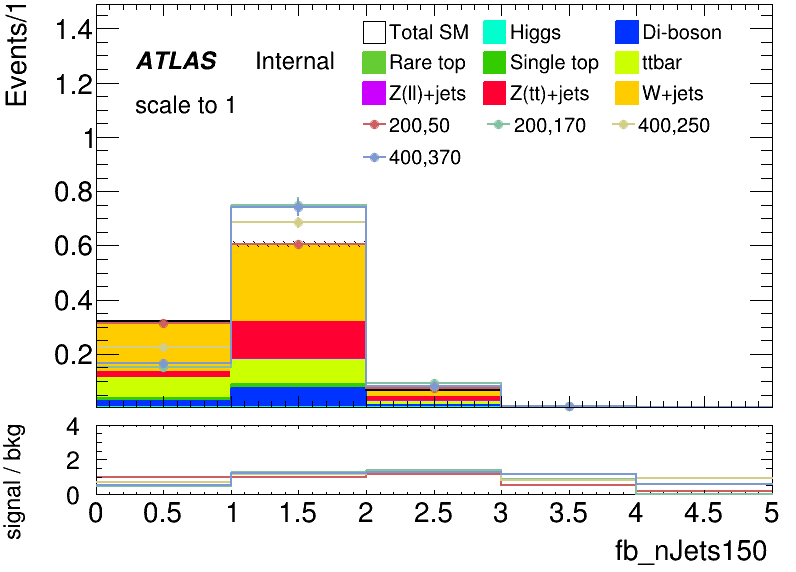
\includegraphics[width=\textwidth]{graphics/LH_met_sig/LH_fb_nJets150_norm.png}
    \end{minipage}
    \hfill
    \begin{minipage}{0.25\textwidth}
        \centering
        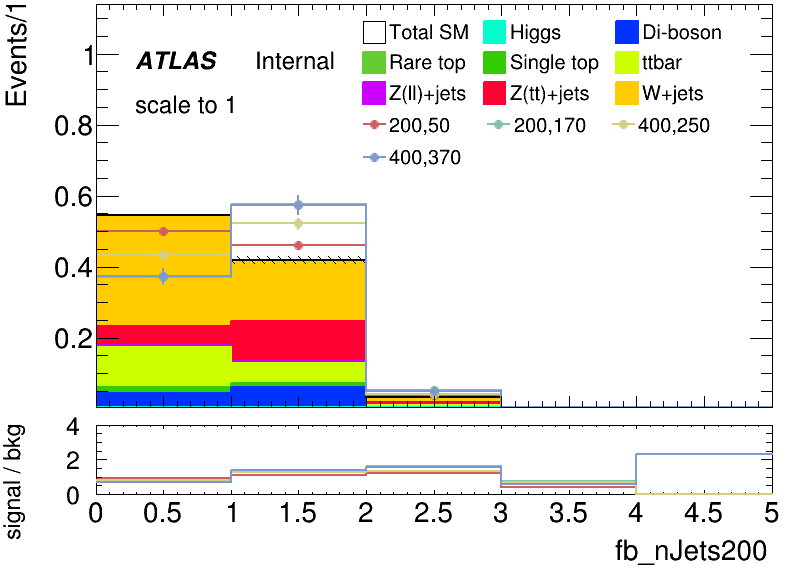
\includegraphics[width=\textwidth]{graphics/LH_met_sig/LH_fb_nJets200_norm.png}
    \end{minipage}
     
    \vspace{0.5cm} % 图片之间的竖直间距

    % 第二行
    \begin{minipage}{0.32\textwidth}
        \centering
        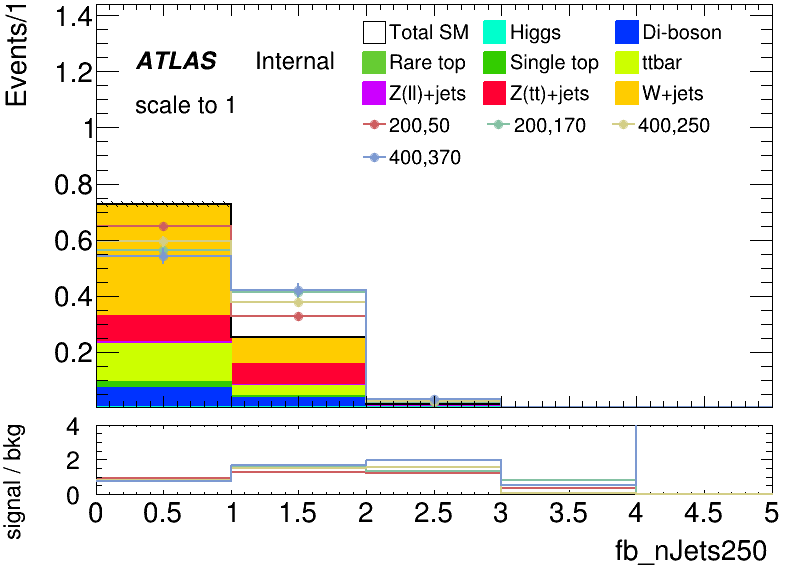
\includegraphics[width=\textwidth]{graphics/LH_met_sig/LH_fb_nJets250_norm.png}
    \end{minipage}
    \hfill
    \begin{minipage}{0.32\textwidth}
        \centering
        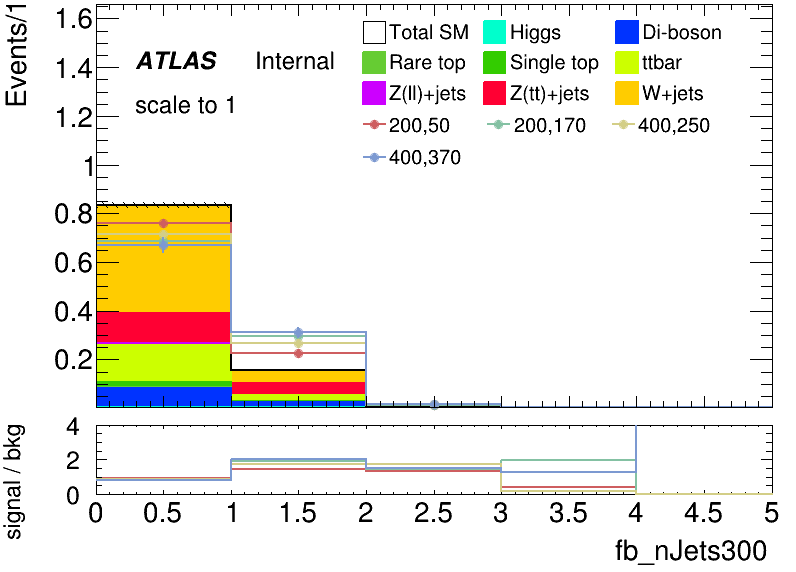
\includegraphics[width=\textwidth]{graphics/LH_met_sig/LH_fb_nJets300_norm.png}
    \end{minipage}
    \hfill
    \begin{minipage}{0.32\textwidth}
        \centering
        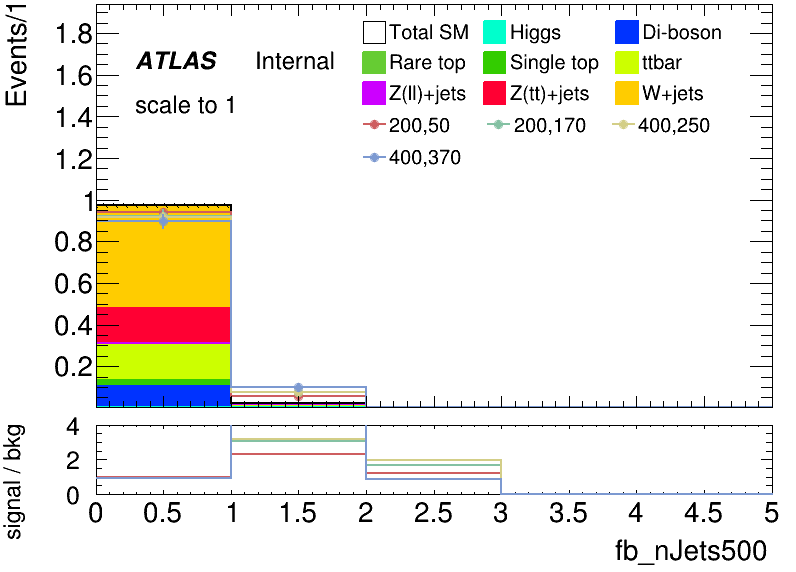
\includegraphics[width=\textwidth]{graphics/LH_met_sig/LH_fb_nJets500_norm.png}
    \end{minipage}
\end{frame}

\begin{frame}

	\frametitle{kinematic distribution}
	\framesubtitle{LH:$m_{inv}$}
    \begin{minipage}{0.32\textwidth}
        \centering
        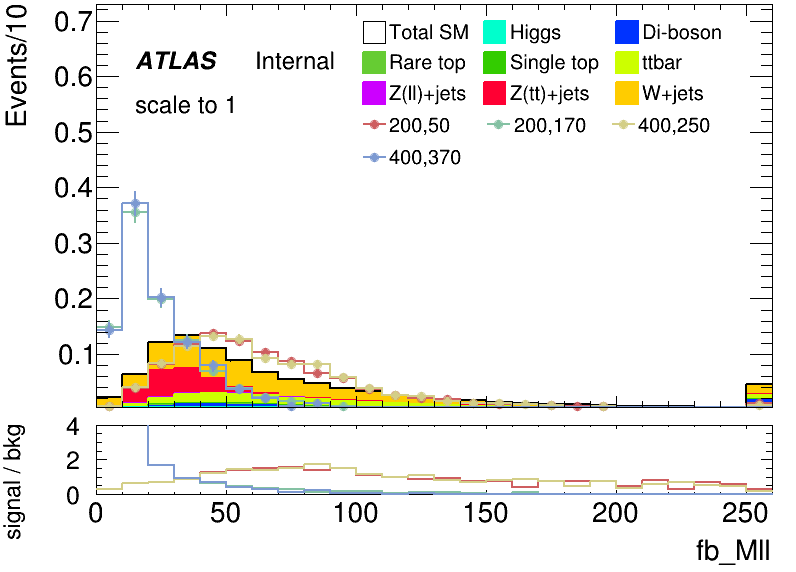
\includegraphics[width=\textwidth]{graphics/LH_met_sig/LH_fb_Mll_norm.png}
    \end{minipage}
    \hfill
    \begin{minipage}{0.32\textwidth}
        \centering
        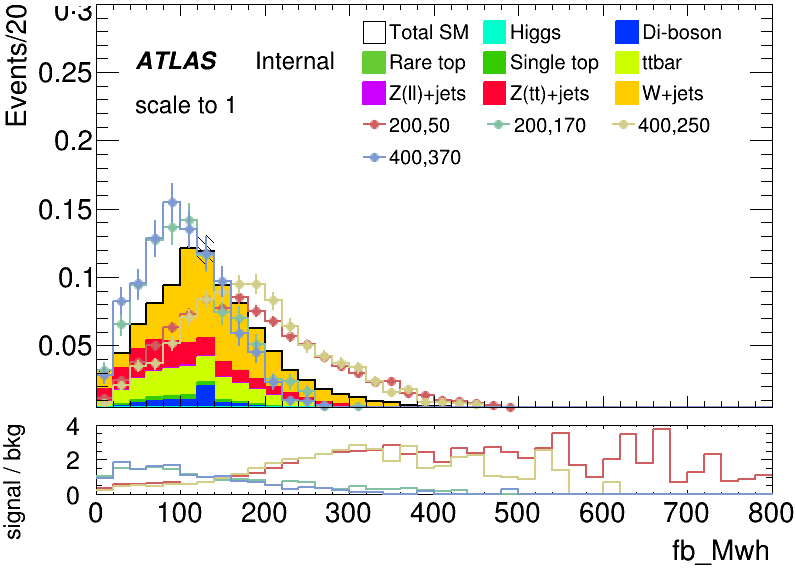
\includegraphics[width=\textwidth]{graphics/LH_met_sig/LH_fb_Mwh_norm.png}
    \end{minipage}
    \hfill
    \begin{minipage}{0.32\textwidth}
        \centering
        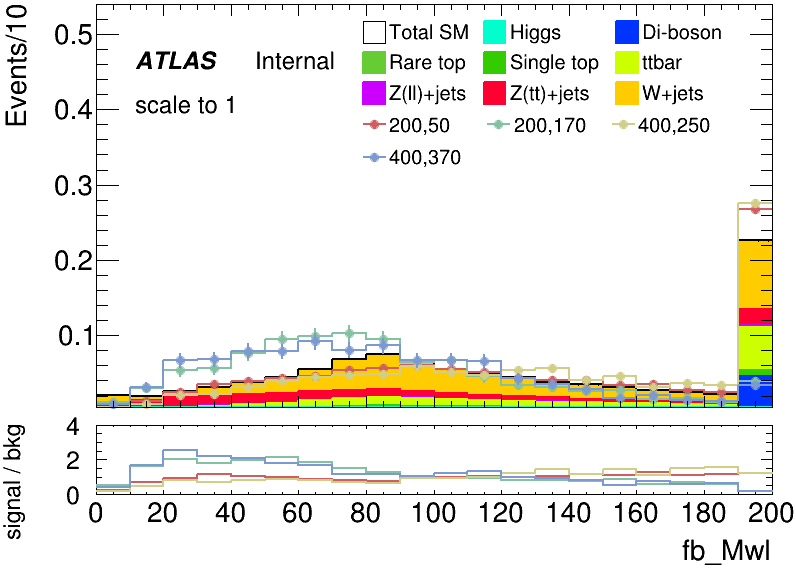
\includegraphics[width=\textwidth]{graphics/LH_met_sig/LH_fb_Mwl_norm.png}
    \end{minipage}	
notice:Mll is invariant between tau1 and tau2, Mwh is invariant between tau1 and MET, Mwl is invariant between tau2 and MET  
\end{frame}

\begin{frame}
	\frametitle{kinematic distribution}
	\framesubtitle{LH:transverse mass}
	    \begin{minipage}{0.25\textwidth}
        \centering
        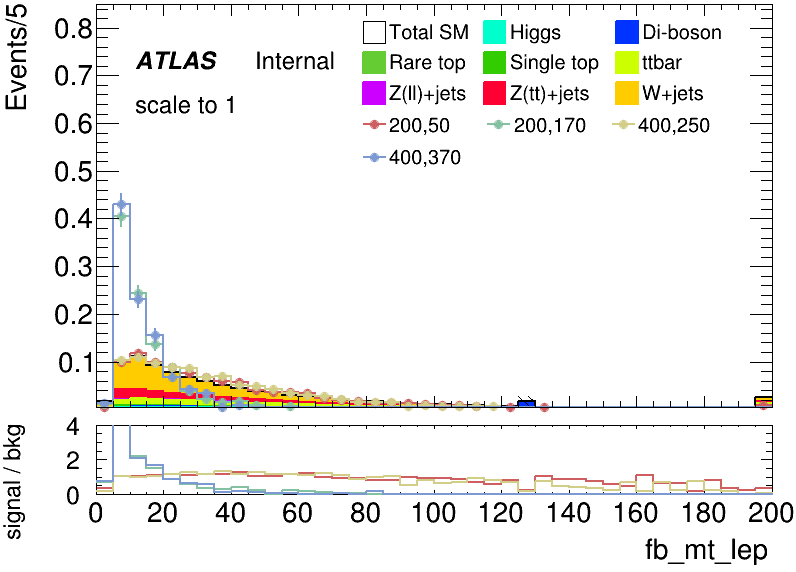
\includegraphics[width=\textwidth]{graphics/LH_met_sig/LH_fb_mt_lep_norm.png}
    \end{minipage}
    \hfill
    \begin{minipage}{0.25\textwidth}
        \centering
        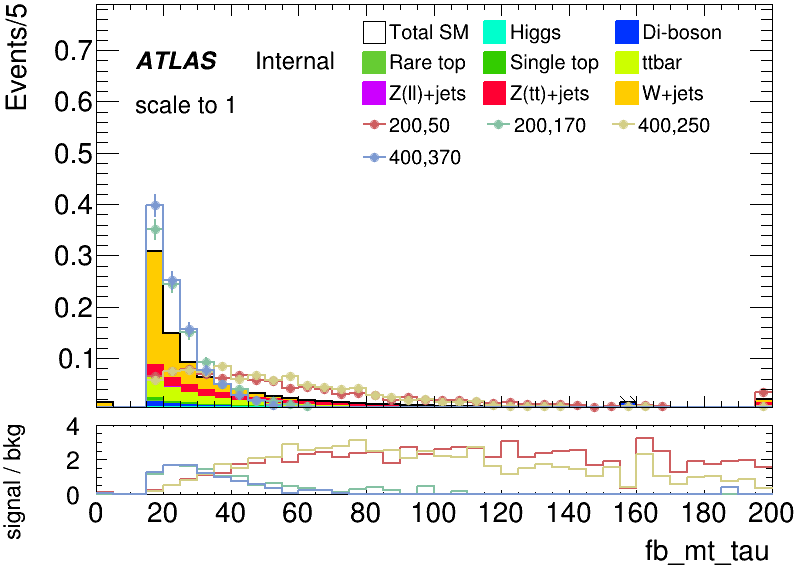
\includegraphics[width=\textwidth]{graphics/LH_met_sig/LH_fb_mt_tau_norm.png}
    \end{minipage}
    \hfill
    \begin{minipage}{0.25\textwidth}
        \centering
        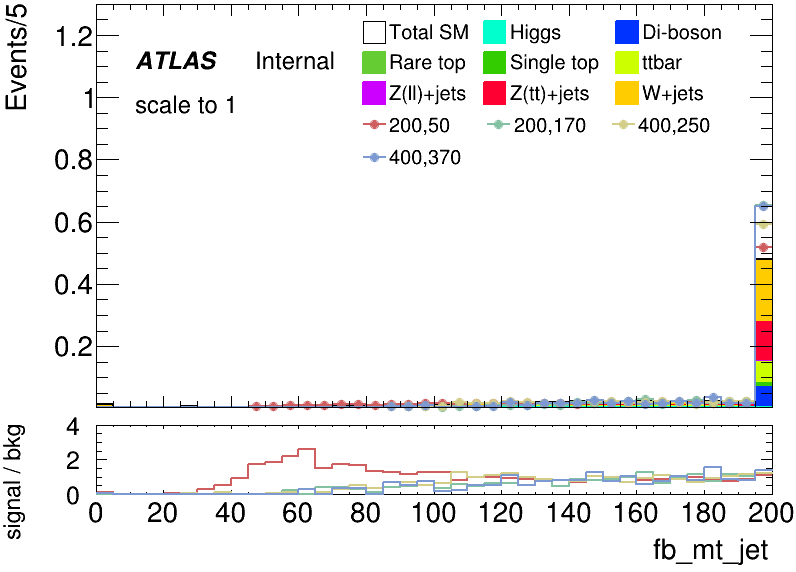
\includegraphics[width=\textwidth]{graphics/LH_met_sig/LH_fb_mt_jet_norm.png}
    \end{minipage}
    \hfill
    \begin{minipage}{0.25\textwidth}
        \centering
        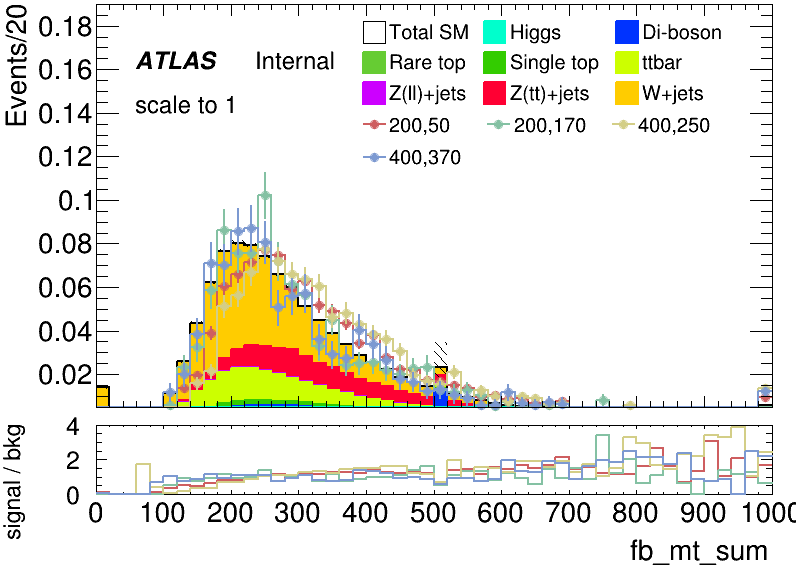
\includegraphics[width=\textwidth]{graphics/LH_met_sig/LH_fb_mt_sum_norm.png}
    \end{minipage}
\end{frame}
\begin{frame}
\frametitle{kinematic distribution}
\framesubtitle{LH:MT2}
    \begin{minipage}{0.32\textwidth}
        \centering
        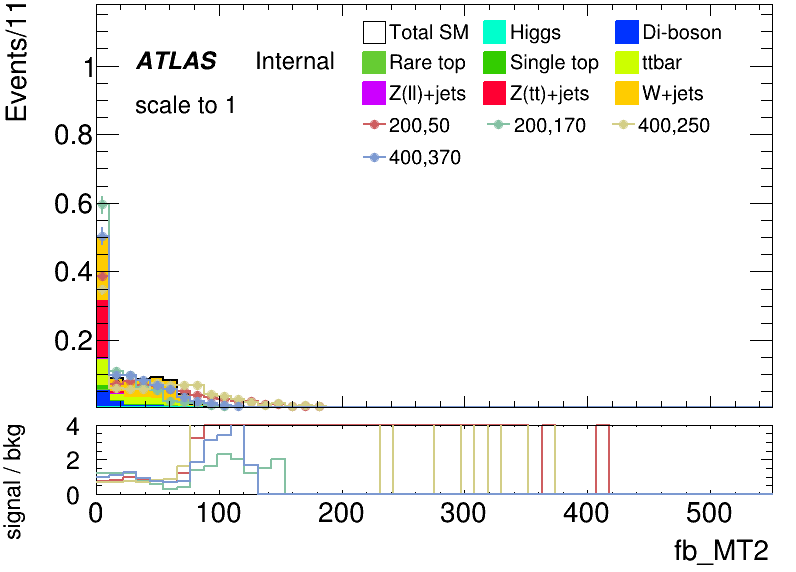
\includegraphics[width=\textwidth]{graphics/LH_met_sig/LH_fb_MT2_norm.png}
    \end{minipage}
    \hfill
    \begin{minipage}{0.32\textwidth}
        \centering
        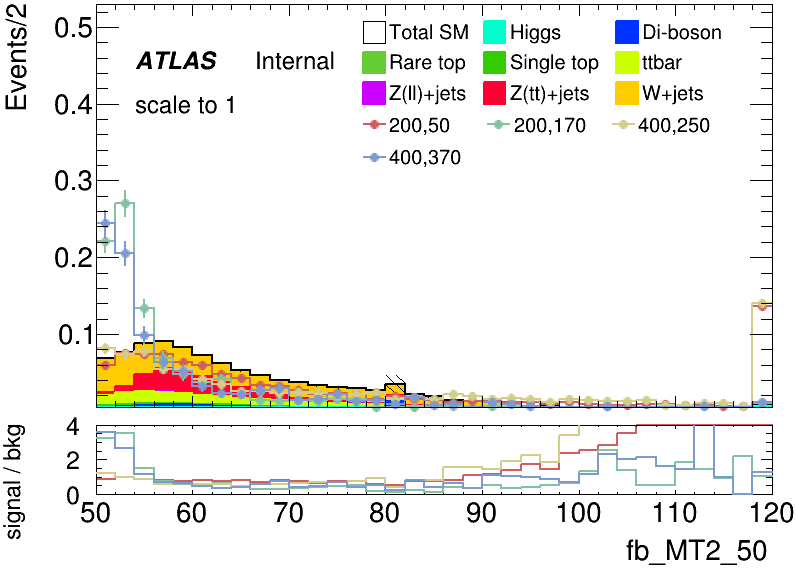
\includegraphics[width=\textwidth]{graphics/LH_met_sig/LH_fb_MT2_50_norm.png}
    \end{minipage}
    \hfill
    \begin{minipage}{0.32\textwidth}
        \centering
        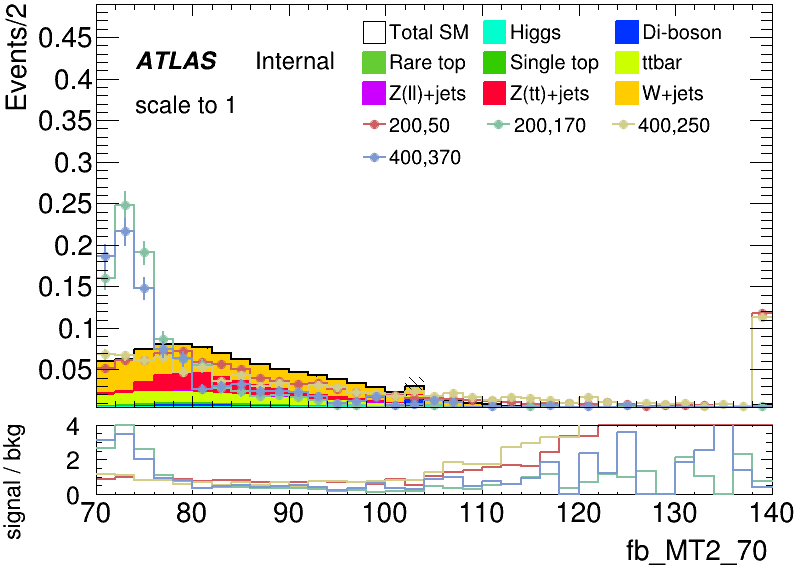
\includegraphics[width=\textwidth]{graphics/LH_met_sig/LH_fb_MT2_70_norm.png}
    \end{minipage}
    
    \vspace{0.5cm}

    \begin{minipage}{0.32\textwidth}
        \centering
        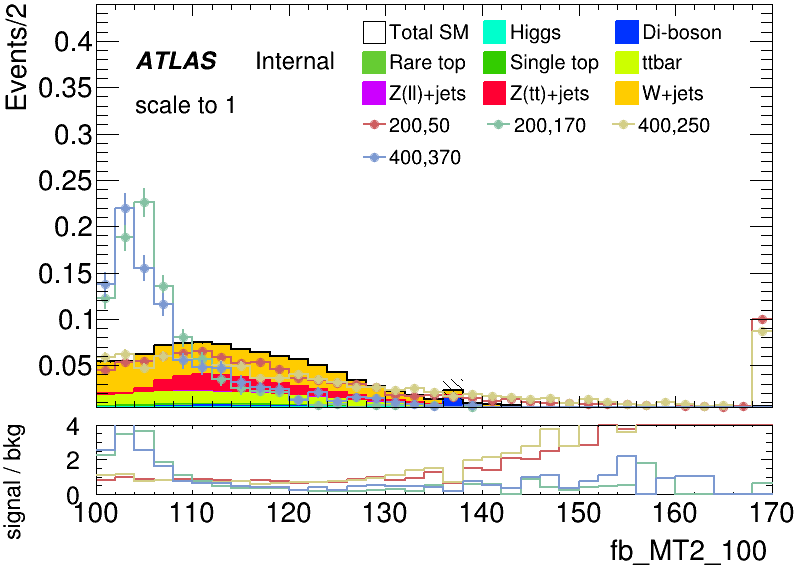
\includegraphics[width=\textwidth]{graphics/LH_met_sig/LH_fb_MT2_100_norm.png}
    \end{minipage}
    \hfill
    \begin{minipage}{0.32\textwidth}
        \centering
        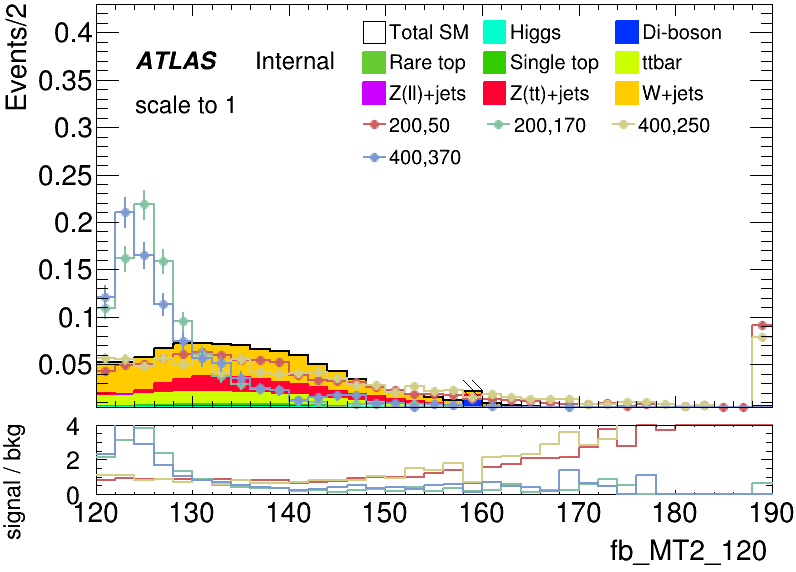
\includegraphics[width=\textwidth]{graphics/LH_met_sig/LH_fb_MT2_120_norm.png}
    \end{minipage}
    \hfill
    \begin{minipage}{0.32\textwidth}
        \centering
        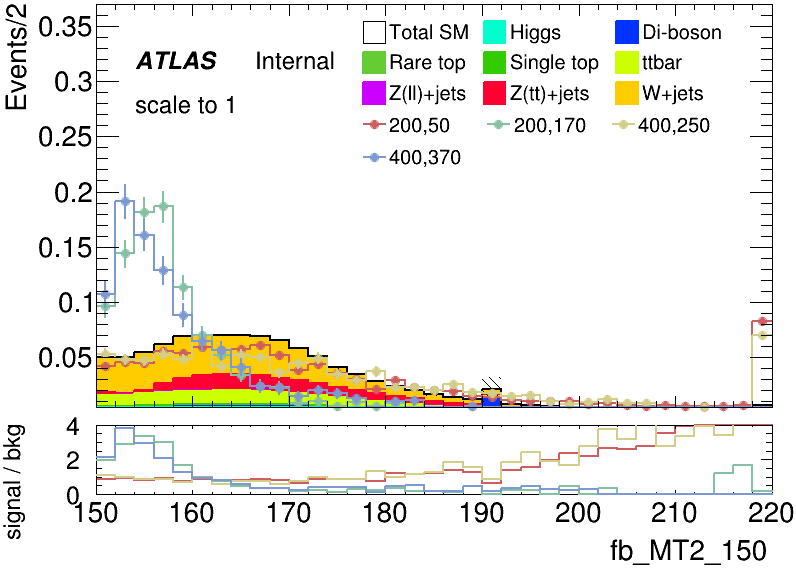
\includegraphics[width=\textwidth]{graphics/LH_met_sig/LH_fb_MT2_150_norm.png}
    \end{minipage}
\end{frame}

\begin{frame}
	\frametitle{kinematic distribution}
	\framesubtitle{LH:ratio}
    \begin{minipage}{0.32\textwidth}
        \centering
        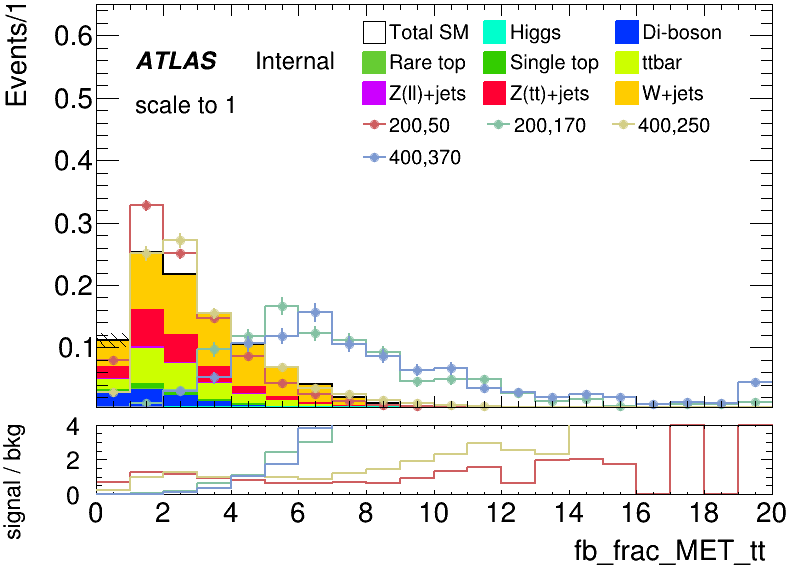
\includegraphics[width=\textwidth]{graphics/LH_met_sig/LH_fb_frac_MET_tt_norm.png}
    \end{minipage}
    \hfill
    \begin{minipage}{0.32\textwidth}
        \centering
        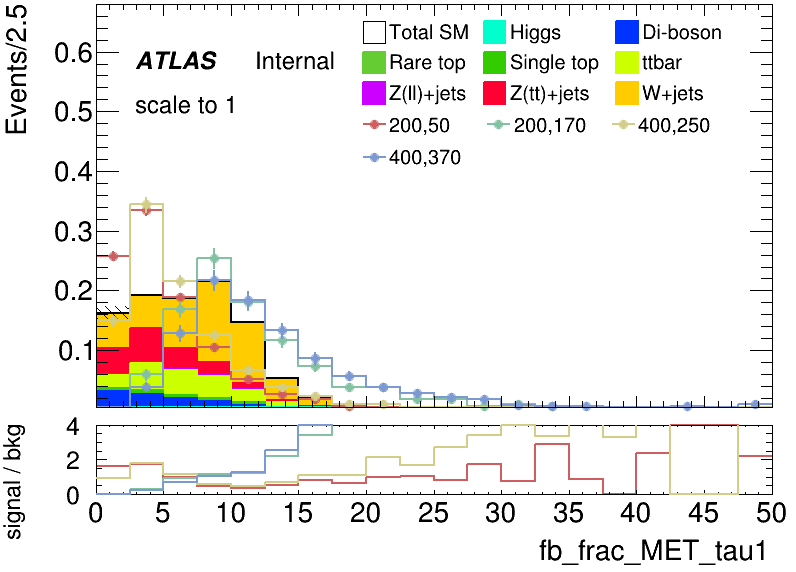
\includegraphics[width=\textwidth]{graphics/LH_met_sig/LH_fb_frac_MET_tau1_norm.png}
    \end{minipage}
    \hfill
    \begin{minipage}{0.32\textwidth}
        \centering
        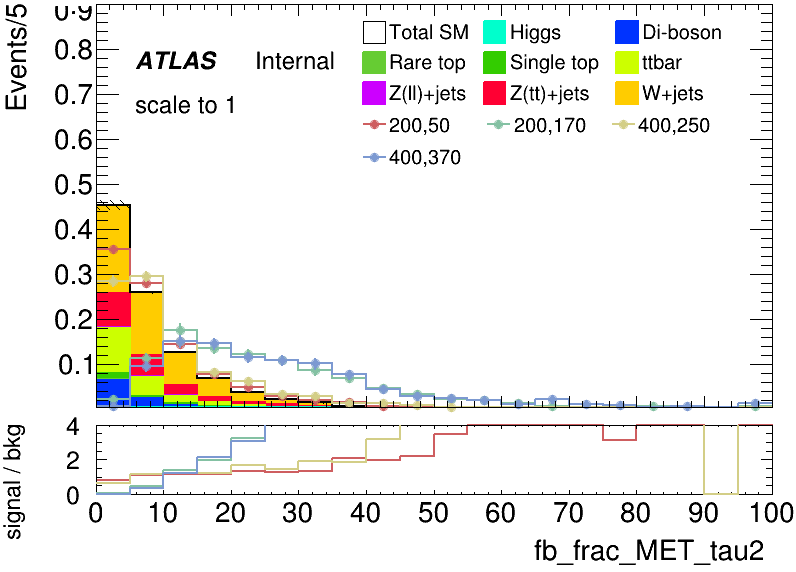
\includegraphics[width=\textwidth]{graphics/LH_met_sig/LH_fb_frac_MET_tau2_norm.png}
    \end{minipage}
    
    \vspace{0.5cm}

    \begin{minipage}{0.32\textwidth}
        \centering
        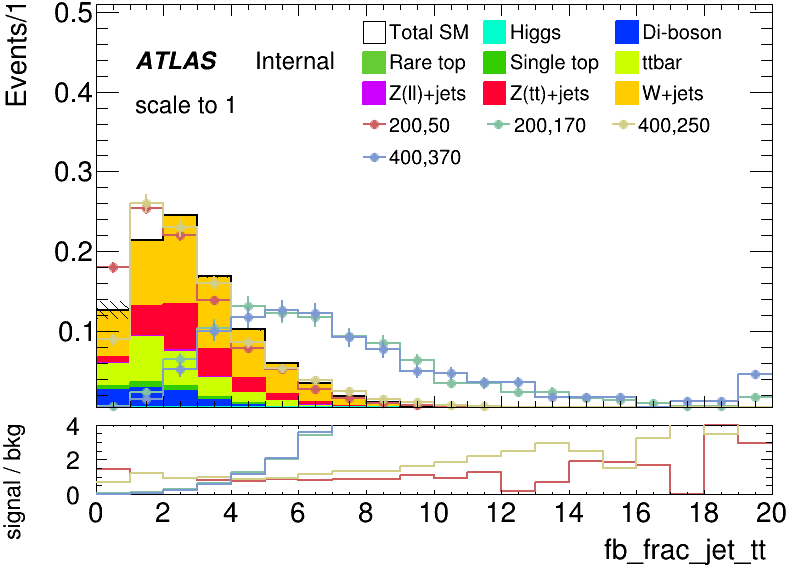
\includegraphics[width=\textwidth]{graphics/LH_met_sig/LH_fb_frac_jet_tt_norm.png}
    \end{minipage}
    \hfill
    \begin{minipage}{0.32\textwidth}
        \centering
        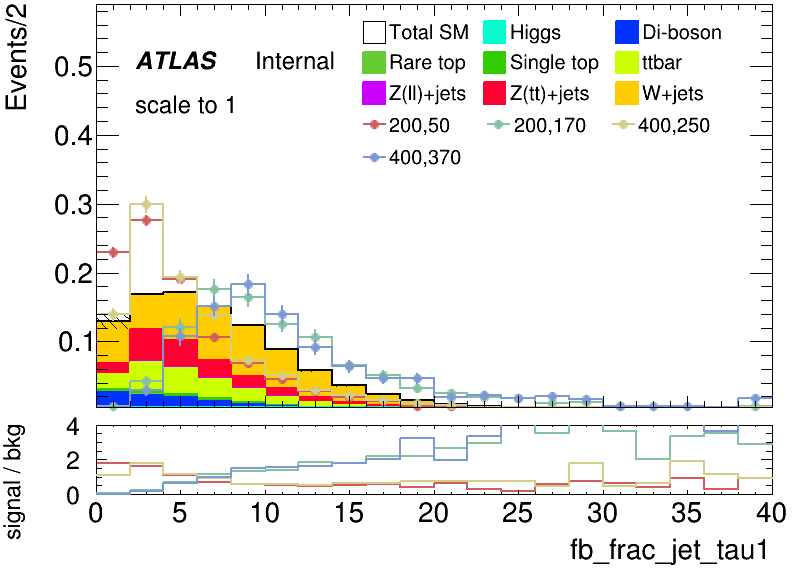
\includegraphics[width=\textwidth]{graphics/LH_met_sig/LH_fb_frac_jet_tau1_norm.png}
    \end{minipage}
    \hfill
    \begin{minipage}{0.32\textwidth}
        \centering
        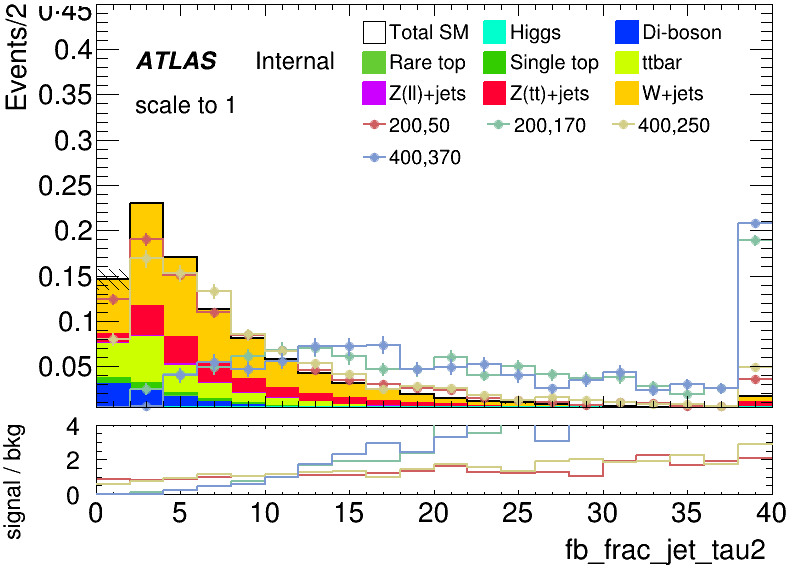
\includegraphics[width=\textwidth]{graphics/LH_met_sig/LH_fb_frac_jet_tau2_norm.png}
    \end{minipage}	
\end{frame}

\begin{frame}
  \frametitle{kinematic distribution}
  \frametitle{LH:$\Delta R$}
    \begin{minipage}{0.32\textwidth}
        \centering
        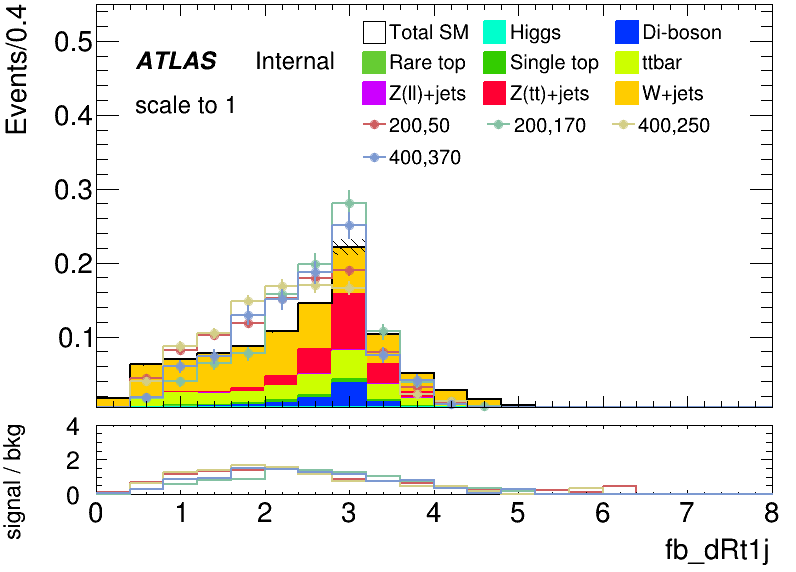
\includegraphics[width=\textwidth]{graphics/LH_met_sig/LH_fb_dRt1j_norm.png}
    \end{minipage}
    \hfill
    \begin{minipage}{0.32\textwidth}
        \centering
        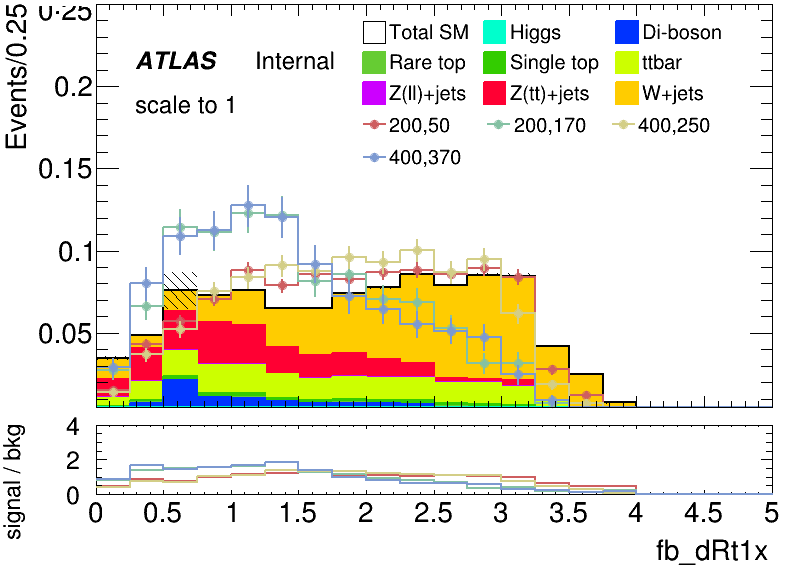
\includegraphics[width=\textwidth]{graphics/LH_met_sig/LH_fb_dRt1x_norm.png}
    \end{minipage}
    \hfill
    \begin{minipage}{0.32\textwidth}
        \centering
        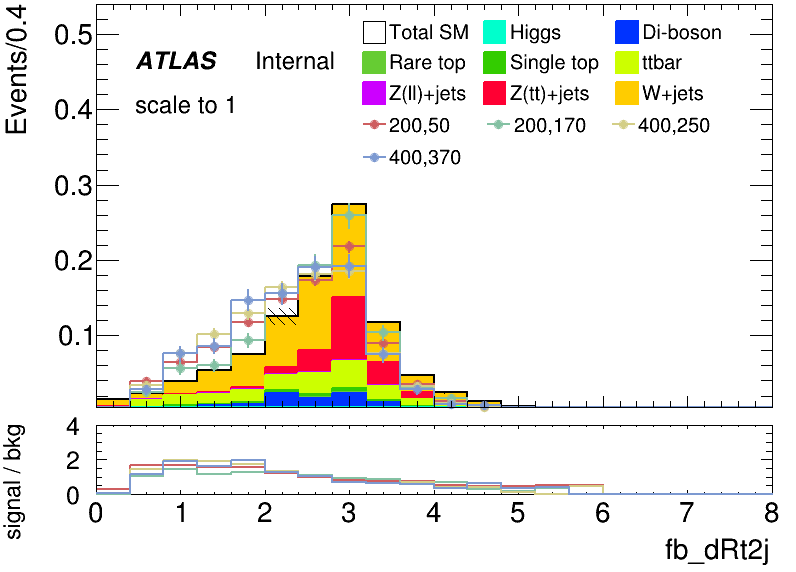
\includegraphics[width=\textwidth]{graphics/LH_met_sig/LH_fb_dRt2j_norm.png}
    \end{minipage}
    
    \vspace{0.5cm} % 图片之间的竖直间距

    % 第二行
    \begin{minipage}{0.32\textwidth}
        \centering
        \includegraphics[width=\textwidth]{graphics/LH_met_sig/LH_fb_dRt2x_norm.png}
    \end{minipage}
    \hfill
    \begin{minipage}{0.32\textwidth}
        \centering
        \includegraphics[width=\textwidth]{graphics/LH_met_sig/LH_fb_dRxj_norm.png}
    \end{minipage}
    \hfill
    \begin{minipage}{0.32\textwidth}
        \centering
        \includegraphics[width=\textwidth]{graphics/LH_met_sig/LH_fb_dRtt_norm.png}
    \end{minipage}
    notice: t1 is leading tau, t2 is leading lep, j is leading jet, x is MET.
\end{frame}

\begin{frame}
  \frametitle{kinematic distribution}
  \framesubtitle{LH:$\Delta\phi$}
    \begin{minipage}{0.32\textwidth}
        \centering
        \includegraphics[width=\textwidth]{graphics/LH_met_sig/LH_fb_dPhit1j_norm.png}
    \end{minipage}
    \hfill
    \begin{minipage}{0.32\textwidth}
        \centering
        \includegraphics[width=\textwidth]{graphics/LH_met_sig/LH_fb_dPhit1x_norm.png}
    \end{minipage}
    \hfill
    \begin{minipage}{0.32\textwidth}
        \centering
        \includegraphics[width=\textwidth]{graphics/LH_met_sig/LH_fb_dPhit2j_norm.png}
    \end{minipage}
    
    \vspace{0.5cm} % 图片之间的竖直间距

    % 第二行
    \begin{minipage}{0.32\textwidth}
        \centering
        \includegraphics[width=\textwidth]{graphics/LH_met_sig/LH_fb_dPhit2x_norm.png}
    \end{minipage}
    \hfill
    \begin{minipage}{0.32\textwidth}
        \centering
        \includegraphics[width=\textwidth]{graphics/LH_met_sig/LH_fb_dPhixj_norm.png}
    \end{minipage}
    \hfill
    \begin{minipage}{0.32\textwidth}
        \centering
        \includegraphics[width=\textwidth]{graphics/LH_met_sig/LH_fb_dPhitt_norm.png}
    \end{minipage}
    notice: t1 is leading tau, t2 is leading lep, j is leading jet, x is MET.
\end{frame}

\section{problems and TODO}
\begin{frame}
	\frametitle{problems and TODO}
	\framesubtitle{problems}
\end{frame}


\section{backup}
\subsection{var definition}
\begin{frame}
	\frametitle{backup}
	The definition of rapidity is $y = \frac{1}{2}ln\frac{E+p_z}{E-p_z}$. $\eta$ is pseudo-rapidity, $\eta = -ln(tan(\frac{\theta}{2})).$ It's easy to detect, and when speed close to light-speed, pseudo-rapidity nearly equal rapidity which can simplify detect of rapidity.
	
	$\phi$ is azimuthal angle of cylindrical coordinates
	
	R is angular distance, $R = \sqrt{\Delta\phi^2+\Delta\eta^2}$, R usually use to judge which particle belong to the same jet.
	
	METsig is Missing Transverse Energy Significance, $METsig = \frac{MET}{\sigma_{MET}}$, $\sigma_{MET}$ is the uncertainty of MET.
	
	Mll is the invariant between two taus, $Mll = \sqrt{(E_1 + E_2)^2 - (\vec{p_1}+\vec{p_2})^2}$
\end{frame}

\subsection{LH MC modeling}
\begin{frame}
\frametitle{C1N2ISR:MC modeling}
\framesubtitle{LH:\quad $\Delta\eta$}
% 第一行
    \begin{minipage}{0.32\textwidth}
        \centering
        \includegraphics[width=\textwidth]{graphics/LH_met/LH_met_dEtat1j.png}
    \end{minipage}
    \hfill
    \begin{minipage}{0.32\textwidth}
        \centering
        \includegraphics[width=\textwidth]{graphics/LH_met/LH_met_dEtat2j.png}
    \end{minipage}
    \hfill
    \begin{minipage}{0.32\textwidth}
        \centering
        \includegraphics[width=\textwidth]{graphics/LH_met/LH_met_dEtatt.png}
    \end{minipage}
    
    \vspace{0.5cm} % 图片之间的竖直间距
    
    notice: t1 is leading tau, t2 is leading lep, j is leading jet, x is MET.
\end{frame}

\begin{frame}
\frametitle{C1N2ISR:MC modeling}
\framesubtitle{LH:\quad $\Delta\phi$}
% 第一行
    \begin{minipage}{0.32\textwidth}
        \centering
        \includegraphics[width=\textwidth]{graphics/LH_met/LH_met_dPhit1j.png}
    \end{minipage}
    \hfill
    \begin{minipage}{0.32\textwidth}
        \centering
        \includegraphics[width=\textwidth]{graphics/LH_met/LH_met_dPhit1x.png}
    \end{minipage}
    \hfill
    \begin{minipage}{0.32\textwidth}
        \centering
        \includegraphics[width=\textwidth]{graphics/LH_met/LH_met_dPhit2j.png}
    \end{minipage}
    
    \vspace{0.5cm} % 图片之间的竖直间距

    % 第二行
    \begin{minipage}{0.32\textwidth}
        \centering
        \includegraphics[width=\textwidth]{graphics/LH_met/LH_met_dPhit2x.png}
    \end{minipage}
    \hfill
    \begin{minipage}{0.32\textwidth}
        \centering
        \includegraphics[width=\textwidth]{graphics/LH_met/LH_met_dPhixj.png}
    \end{minipage}
    \hfill
    \begin{minipage}{0.32\textwidth}
        \centering
        \includegraphics[width=\textwidth]{graphics/LH_met/LH_met_dPhitt.png}
    \end{minipage}
    notice: t1 is leading tau, t2 is leading lep, j is leading jet, x is MET.
\end{frame}

\begin{frame}
\frametitle{C1N2ISR:MC modeling}
\framesubtitle{LH:\quad $\Delta R$}
% 第一行
    \begin{minipage}{0.32\textwidth}
        \centering
        \includegraphics[width=\textwidth]{graphics/LH_met/LH_met_dRt1j.png}
    \end{minipage}
    \hfill
    \begin{minipage}{0.32\textwidth}
        \centering
        \includegraphics[width=\textwidth]{graphics/LH_met/LH_met_dRt1x.png}
    \end{minipage}
    \hfill
    \begin{minipage}{0.32\textwidth}
        \centering
        \includegraphics[width=\textwidth]{graphics/LH_met/LH_met_dRt2j.png}
    \end{minipage}
    
    \vspace{0.5cm} % 图片之间的竖直间距

    % 第二行
    \begin{minipage}{0.32\textwidth}
        \centering
        \includegraphics[width=\textwidth]{graphics/LH_met/LH_met_dRt2x.png}
    \end{minipage}
    \hfill
    \begin{minipage}{0.32\textwidth}
        \centering
        \includegraphics[width=\textwidth]{graphics/LH_met/LH_met_dRxj.png}
    \end{minipage}
    \hfill
    \begin{minipage}{0.32\textwidth}
        \centering
        \includegraphics[width=\textwidth]{graphics/LH_met/LH_met_dRtt.png}
    \end{minipage}
    notice: t1 is leading tau, t2 is leading lep, j is leading jet, x is MET.
\end{frame}

\begin{frame}
\frametitle{C1N2ISR:MC modeling}
\framesubtitle{LH:$\quad\eta$}
% 第一行
    \begin{minipage}{0.32\textwidth}
        \centering
        \includegraphics[width=\textwidth]{graphics/LH_met/LH_met_eta_jet.png}
    \end{minipage}
    \hfill
    \begin{minipage}{0.32\textwidth}
        \centering
        \includegraphics[width=\textwidth]{graphics/LH_met/LH_met_eta_lep.png}
    \end{minipage}
    \hfill
    \begin{minipage}{0.32\textwidth}
        \centering
        \includegraphics[width=\textwidth]{graphics/LH_met/LH_met_eta_tau.png}
    \end{minipage}
\end{frame}

\begin{frame}
\frametitle{C1N2ISR:MC modeling}
\framesubtitle{LH:\quad $p_t$}
% 第一行
    \begin{minipage}{0.32\textwidth}
        \centering
        \includegraphics[width=\textwidth]{graphics/LH_met/LH_met_pt_jet.png}
    \end{minipage}
    \hfill
    \begin{minipage}{0.32\textwidth}
        \centering
        \includegraphics[width=\textwidth]{graphics/LH_met/LH_met_pt_lep.png}
    \end{minipage}
    \hfill
    \begin{minipage}{0.32\textwidth}
        \centering
        \includegraphics[width=\textwidth]{graphics/LH_met/LH_met_pt_tau.png}
    \end{minipage}
    
    \vspace{0.5cm} % 图片之间的竖直间距
\end{frame}

\begin{frame}
\frametitle{C1N2ISR:MC modeling}
\framesubtitle{LH:\quad num}
% 第一行
    \begin{minipage}{0.32\textwidth}
        \centering
        \includegraphics[width=\textwidth]{graphics/LH_met/LH_met_nEles.png}
    \end{minipage}
    \hfill
    \begin{minipage}{0.32\textwidth}
        \centering
        \includegraphics[width=\textwidth]{graphics/LH_met/LH_met_nJets.png}
    \end{minipage}
    \hfill
    \begin{minipage}{0.32\textwidth}
        \centering
        \includegraphics[width=\textwidth]{graphics/LH_met/LH_met_nLeps.png}
    \end{minipage}
    
    \vspace{0.5cm} % 图片之间的竖直间距

    % 第二行
    \begin{minipage}{0.32\textwidth}
        \centering
        \includegraphics[width=\textwidth]{graphics/LH_met/LH_met_nMuons.png}
    \end{minipage}
    \hfill
    \begin{minipage}{0.32\textwidth}
        \centering
        \includegraphics[width=\textwidth]{graphics/LH_met/LH_met_nTaus.png}
    \end{minipage}
    \hfill
    \begin{minipage}{0.32\textwidth}
        \centering
        \includegraphics[width=\textwidth]{graphics/LH_met/LH_met_nTightTaus.png}
    \end{minipage}
\end{frame}

\begin{frame}
\frametitle{C1N2ISR:MC modeling}
\framesubtitle{LH:\quad transverse mass}
% 第一行
    \begin{minipage}{0.32\textwidth}
        \centering
        \includegraphics[width=\textwidth]{graphics/LH_met/LH_met_mt_jet.png}
    \end{minipage}
    \hfill
    \begin{minipage}{0.32\textwidth}
        \centering
        \includegraphics[width=\textwidth]{graphics/LH_met/LH_met_mt_lep.png}
    \end{minipage}
    \hfill
    \begin{minipage}{0.32\textwidth}
        \centering
        \includegraphics[width=\textwidth]{graphics/LH_met/LH_met_mt_tau.png}
    \end{minipage}
    
    \vspace{0.5cm} % 图片之间的竖直间距

    % 第二行
    \begin{minipage}{0.32\textwidth}
        \centering
        \includegraphics[width=\textwidth]{graphics/LH_met/LH_met_mtx_jet.png}
    \end{minipage}
        \hfill
    \begin{minipage}{0.32\textwidth}
        \centering
        \includegraphics[width=\textwidth]{graphics/LH_met/LH_met_mtx_lep.png}
    \end{minipage}
    \hfill
    \begin{minipage}{0.32\textwidth}
        \centering
        \includegraphics[width=\textwidth]{graphics/LH_met/LH_met_mtx_tau.png}
    \end{minipage}
    notice: mtx is the projection of MT in METvec.
\end{frame}
\begin{frame}
\frametitle{C1N2ISR:MC modeling}
\framesubtitle{LH:\quad stranverse mass, invariant mass, MET}
% 第一行
    \begin{minipage}{0.32\textwidth}
        \centering
        \includegraphics[width=\textwidth]{graphics/LH_met/LH_met_Mll.png}
    \end{minipage}
    \hfill
    \begin{minipage}{0.32\textwidth}
        \centering
        \includegraphics[width=\textwidth]{graphics/LH_met/LH_met_MT2.png}
    \end{minipage}
    \hfill
%    \begin{minipage}{0.32\textwidth}
%        \centering
%        \includegraphics[width=\textwidth]{graphics/H_met/H_met_dPhit2j.png}
%    \end{minipage}
    
    \vspace{0.5cm} % 图片之间的竖直间距

    % 第二行
    \begin{minipage}{0.32\textwidth}
        \centering
        \includegraphics[width=\textwidth]{graphics/LH_met/LH_met_MET.png}
    \end{minipage}
    \hfill
    \begin{minipage}{0.32\textwidth}
        \centering
        \includegraphics[width=\textwidth]{graphics/LH_met/LH_met_METsig.png}
    \end{minipage}
    \hfill
    
%    \begin{minipage}{0.32\textwidth}
%        \centering
%        \includegraphics[width=\textwidth]{graphics/H_met/H_met_dPhitt.png}
%    \end{minipage}

\end{frame}

\subsection{HH MC modeling}
\begin{frame}
\frametitle{C1N2ISR:MC modeling}
\framesubtitle{HH:\quad $\Delta\eta$}
% 第一行
    \begin{minipage}{0.32\textwidth}
        \centering
        \includegraphics[width=\textwidth]{graphics/HH_met/HH_met_dEtat1j.png}
    \end{minipage}
    \hfill
    \begin{minipage}{0.32\textwidth}
        \centering
        \includegraphics[width=\textwidth]{graphics/HH_met/HH_met_dEtat2j.png}
    \end{minipage}
    \hfill
    \begin{minipage}{0.32\textwidth}
        \centering
        \includegraphics[width=\textwidth]{graphics/HH_met/HH_met_dEtatt.png}
    \end{minipage}
    
    \vspace{0.5cm} % 图片之间的竖直间距\
    notice: t1 is leading tau, t2 is next leading tau, j is leading jet, x is MET.
\end{frame}

\begin{frame}
\frametitle{C1N2ISR:MC modeling}
\framesubtitle{HH:\quad $\Delta\phi$}
% 第一行
    \begin{minipage}{0.32\textwidth}
        \centering
        \includegraphics[width=\textwidth]{graphics/HH_met/HH_met_dPhit1j.png}
    \end{minipage}
    \hfill
    \begin{minipage}{0.32\textwidth}
        \centering
        \includegraphics[width=\textwidth]{graphics/HH_met/HH_met_dPhit1x.png}
    \end{minipage}
    \hfill
    \begin{minipage}{0.32\textwidth}
        \centering
        \includegraphics[width=\textwidth]{graphics/HH_met/HH_met_dPhit2j.png}
    \end{minipage}
    
    \vspace{0.5cm} % 图片之间的竖直间距

    % 第二行
    \begin{minipage}{0.32\textwidth}
        \centering
        \includegraphics[width=\textwidth]{graphics/HH_met/HH_met_dPhit2x.png}
    \end{minipage}
    \hfill
    \begin{minipage}{0.32\textwidth}
        \centering
        \includegraphics[width=\textwidth]{graphics/HH_met/HH_met_dPhixj.png}
    \end{minipage}
    \hfill
    \begin{minipage}{0.32\textwidth}
        \centering
        \includegraphics[width=\textwidth]{graphics/HH_met/HH_met_dPhitt.png}
    \end{minipage}
    notice: t1 is leading tau, t2 is next leading tau, j is leading jet, x is MET.
\end{frame}

\begin{frame}
\frametitle{C1N2ISR:MC modeling}
\framesubtitle{HH:\quad $\Delta R$}
% 第一行
    \begin{minipage}{0.32\textwidth}
        \centering
        \includegraphics[width=\textwidth]{graphics/HH_met/HH_met_dRt1j.png}
    \end{minipage}
    \hfill
    \begin{minipage}{0.32\textwidth}
        \centering
        \includegraphics[width=\textwidth]{graphics/HH_met/HH_met_dRt1x.png}
    \end{minipage}
    \hfill
    \begin{minipage}{0.32\textwidth}
        \centering
        \includegraphics[width=\textwidth]{graphics/HH_met/HH_met_dRt2j.png}
    \end{minipage}
    
    \vspace{0.5cm} % 图片之间的竖直间距

    % 第二行
    \begin{minipage}{0.32\textwidth}
        \centering
        \includegraphics[width=\textwidth]{graphics/HH_met/HH_met_dRt2x.png}
    \end{minipage}
    \hfill
    \begin{minipage}{0.32\textwidth}
        \centering
        \includegraphics[width=\textwidth]{graphics/HH_met/HH_met_dRxj.png}
    \end{minipage}
    \hfill
    \begin{minipage}{0.32\textwidth}
        \centering
        \includegraphics[width=\textwidth]{graphics/HH_met/HH_met_dRtt.png}
    \end{minipage}
    notice: t1 is leading tau, t2 is next leading tau, j is leading jet, x is MET.
\end{frame}

\begin{frame}
\frametitle{C1N2ISR:MC modeling}
\framesubtitle{HH:$\quad\eta$}
% 第一行
    \begin{minipage}{0.32\textwidth}
        \centering
        \includegraphics[width=\textwidth]{graphics/HH_met/HH_met_eta_jet.png}
    \end{minipage}
    \hfill
    \begin{minipage}{0.32\textwidth}
        \centering
        \includegraphics[width=\textwidth]{graphics/HH_met/HH_met_eta_lep.png}
    \end{minipage}
    \hfill
    \begin{minipage}{0.32\textwidth}
        \centering
        \includegraphics[width=\textwidth]{graphics/HH_met/HH_met_eta_tau.png}
    \end{minipage}
    notice: jet is leading jet, lep is next leading tau, tau is leading tau.
\end{frame}

\begin{frame}
\frametitle{C1N2ISR:MC modeling}
\framesubtitle{HH:\quad $p_t$}
% 第一行
    \begin{minipage}{0.32\textwidth}
        \centering
        \includegraphics[width=\textwidth]{graphics/HH_met/HH_met_pt_jet.png}
    \end{minipage}
    \hfill
    \begin{minipage}{0.32\textwidth}
        \centering
        \includegraphics[width=\textwidth]{graphics/HH_met/HH_met_pt_lep.png}
    \end{minipage}
    \hfill
    \begin{minipage}{0.32\textwidth}
        \centering
        \includegraphics[width=\textwidth]{graphics/HH_met/HH_met_pt_tau.png}
    \end{minipage}
    
    \vspace{0.5cm} % 图片之间的竖直间距
    notice: jet is leading jet, lep is next leading tau, tau is leading tau.
\end{frame}

\begin{frame}
\frametitle{C1N2ISR:MC modeling}
\framesubtitle{HH:\quad num}
% 第一行
    \begin{minipage}{0.32\textwidth}
        \centering
        \includegraphics[width=\textwidth]{graphics/HH_met/HH_met_nEles.png}
    \end{minipage}
    \hfill
    \begin{minipage}{0.32\textwidth}
        \centering
        \includegraphics[width=\textwidth]{graphics/HH_met/HH_met_nJets.png}
    \end{minipage}
    \hfill
    \begin{minipage}{0.32\textwidth}
        \centering
        \includegraphics[width=\textwidth]{graphics/HH_met/HH_met_nLeps.png}
    \end{minipage}
    
    \vspace{0.5cm} % 图片之间的竖直间距

    % 第二行
    \begin{minipage}{0.32\textwidth}
        \centering
        \includegraphics[width=\textwidth]{graphics/HH_met/HH_met_nMuons.png}
    \end{minipage}
    \hfill
    \begin{minipage}{0.32\textwidth}
        \centering
        \includegraphics[width=\textwidth]{graphics/HH_met/HH_met_nTaus.png}
    \end{minipage}
    \hfill
    \begin{minipage}{0.32\textwidth}
        \centering
        \includegraphics[width=\textwidth]{graphics/HH_met/HH_met_nTightTaus.png}
    \end{minipage}
\end{frame}

\begin{frame}
\frametitle{C1N2ISR:MC modeling}
\framesubtitle{HH:\quad transverse mass}
% 第一行
    \begin{minipage}{0.32\textwidth}
        \centering
        \includegraphics[width=\textwidth]{graphics/HH_met/HH_met_mt_jet.png}
    \end{minipage}
    \hfill
    \begin{minipage}{0.32\textwidth}
        \centering
        \includegraphics[width=\textwidth]{graphics/HH_met/HH_met_mt_lep.png}
    \end{minipage}
    \hfill
    \begin{minipage}{0.32\textwidth}
        \centering
        \includegraphics[width=\textwidth]{graphics/HH_met/HH_met_mt_tau.png}
    \end{minipage}
    
    \vspace{0.5cm} % 图片之间的竖直间距

    % 第二行
    \begin{minipage}{0.32\textwidth}
        \centering
        \includegraphics[width=\textwidth]{graphics/HH_met/HH_met_mtx_jet.png}
    \end{minipage}
        \hfill
    \begin{minipage}{0.32\textwidth}
        \centering
        \includegraphics[width=\textwidth]{graphics/HH_met/HH_met_mtx_lep.png}
    \end{minipage}
    \hfill
    \begin{minipage}{0.32\textwidth}
        \centering
        \includegraphics[width=\textwidth]{graphics/HH_met/HH_met_mtx_tau.png}
    \end{minipage}
    notice: mtx is the projection of MT in METvec.
\end{frame}
\begin{frame}
\frametitle{C1N2ISR:MC modeling}
\framesubtitle{HH:\quad stranverse mass, invariant mass, MET}
% 第一行
    \begin{minipage}{0.32\textwidth}
        \centering
        \includegraphics[width=\textwidth]{graphics/HH_met/HH_met_Mll.png}
    \end{minipage}
    \hfill
    \begin{minipage}{0.32\textwidth}
        \centering
        \includegraphics[width=\textwidth]{graphics/HH_met/HH_met_MT2.png}
    \end{minipage}
    \hfill
%    \begin{minipage}{0.32\textwidth}
%        \centering
%        \includegraphics[width=\textwidth]{graphics/H_met/H_met_dPhit2j.png}
%    \end{minipage}
    
    \vspace{0.5cm} % 图片之间的竖直间距

    % 第二行
    \begin{minipage}{0.32\textwidth}
        \centering
        \includegraphics[width=\textwidth]{graphics/HH_met/HH_met_MET.png}
    \end{minipage}
    \hfill
    \begin{minipage}{0.32\textwidth}
        \centering
        \includegraphics[width=\textwidth]{graphics/HH_met/HH_met_METsig.png}
    \end{minipage}
    \hfill
    
%    \begin{minipage}{0.32\textwidth}
%        \centering
%        \includegraphics[width=\textwidth]{graphics/H_met/H_met_dPhitt.png}
%    \end{minipage}

\end{frame}

\end{document}
